\chapter{\label{6ethnographicResults}Ethnographic Results 2}

\minitoc



\section{Abstract}
In this chapter I assess the predictions of this dissertation in light of ethnographic evidence collected with the Beijing Men's rugby team.  Having described the specific cultural terrain of the research context in the previous Chapter (Chapter ~\ref{chap:ethnoField}), the contours of generalisable cognitive mechanisms relevant to the predictions of this dissertation become more visible. I identify three key categories of athlete experience---1) perceptions of performance in joint action, 2) feelings relating to ``team click'', and 3) processes of group membership---which I argue are relevant to the hypothesised relationship between joint action and social bonding, as well as the hypothesised mediating role of team click in this relationship. I also outline evidence for possible moderating variables of these relationships, such as technical competence, personality type, injury, and fatigue. I conclude the chapter by summarising and discussing the results, with a particular focus on how these observations could be operationalised in further experimental studies with a larger sample of athletes beyond the Beijing men's team.





                                      \begin{CJK}{UTF8}{gbsn}
                                        ends




\section{Introduction}

Restate the question: come together and move together

Restate context
Specific terrain (Chap5)
predictions


\section{Analysis of study predictions: Relationship between joint action and social bonding}

In this results section, I outline ethnographic evidence according to the theoretical predictions set out in this dissertation concerning joint action and social bonding. Results are divided into three sections: 1) perceptions of performance in joint action, 2) team click, and 3) group membership




\subsection{Perceptions of performance in joint action}
Unsurprisingly, ethnographic observations revealed that perceptions of performance of on-field requirements of rugby were a central dimension to athletes' experience of the rugby program at the Institute.  As explained in the previous section, most of the athletes in the program at the Institute transitioned from other sports, or otherwise had no specific background in sport before coming to the Institute.  Rugby's minnow status in China means that its technical requirements are not widely known or understood.  Thus, from a very low base of prior knowledge, athletes are forced to develop technical competence in rugby and a fluency in the social environment of the team.  The ability to effectively coordinate behaviour with others, both on and off the field, is therefore crucial to an athlete's ability to navigate the rugby program at the Institute and access the incentives available.

%In addition, the concept of living and training full time with a group of non-kin is, as a general rule, a relatively novel social requirement for most athletes.  Millions of Chinese university aged students leave home and cohabitate in university dormitories, prior to which point most live at home with their immediate families.

%Starting at time with almost zero prior experience of rugby, athletes must learn the technical skills of passing, tackling, running, kicking---and all of these these individual technical components must be harmonised in joint action with other athletes on the same team, as well as against opposition athletes.  Off the field, as discussed in the previous chapter, the rugby program at the Institute requires athletes to navigate a complex social environment, structured by hierarchical relations of power.

\subsubsection{Team Awareness}
During interviews, within the general theme of the costs and benefits of adherence to rugby, I asked athletes what they found to be ``the most difficult part of rugby.''  20 of the 26 athletes interviewed responded directly to the question, and all interpreted it as a question about rugby's technical technical demands.  As unruly undergrad Fang Chao summarised well:

\begin{quotation}
  The hardest thing about rugby is all of the small details. Rugby is such a comprehensive sport, and playing in a real game is very different from training. I remember when was playing a tournament in 2014, at the time I had only just started training (for rugby).  As soon as I took the field my whole brain was blank.  Now I am a bit better, my vision is broader.
\end{quotation}

\begin{quotation}
  橄榄球最难的一部分是很多小细节吧。橄榄球是很全面的项目...打比赛跟训练还是有区别的. 14年的时候打比赛,那时候刚练,一上场整个脑子就空白了,现在会好一点,视野也开阔了
\end{quotation}

Responses indicate that athletes perceive the on-field joint action demands of rugby the most difficult. 11 athletes cited an aspect of rugby that related to on-field coordination of behaviour in joint action, such as decision making in attack, ``awareness'' or vision in game play, coordinating running lines, executing planned plays, and so on.  Seven athletes cited aspects of individual performance, such as tackling, speed in defence, footwork in attack. The remaining two athletes cited both an aspect that was related to coordination of behaviours with others, as well as an aspect of individual performance.
As Wang Zhenfeng, a tall and extremely talented (but inexperienced) senior athlete, explained:

\begin{quotation}
  For me, it's probably the decision making with ball in hand: after you get the ball, how you create opportunities for others---I think that's especially difficult.  For me I think breaking the line or attack or whatever, breaking the line or stepping and so on...I'm ok at all of these things, but if you ask me to create an opportunity for someone else after I have broken the line---that's when I find it difficult.
\end{quotation}

\begin{quotation}
  对我来讲应该是球的分化,拿到球之后分化给别人创造机会我觉得特别难。我觉得突破或进攻还是干嘛的,去突变向什么的对我来说都还好,但是让我即能突然后给别人创造机会我觉得很难。
\end{quotation}

Wang Zhankun, a young and promising kid from Chaoyang school expressed a similar sentiment:

\begin{quotation}
  I’d say the ability to adjust to being on the field in a game.  When I’m on the field I can only see those few people who are close to me, when I’m tired I feel like I can’t see anything, like there could be a gap, or an opportunity, but often I can see it.
\end{quotation}

\begin{quotation}
  场上的适应能力吧。我在场上只能看到离自己近的几个人,累的时候感觉看不到所有,可能空档啊、机会啊经常看不到.
\end{quotation}

The theme of ``awareness'' (\textit{yishi} 意识) was prominent in answers to this question. Of the 13 athletes who cited coordination of behaviour with others as (or one of) the most difficult aspect of rugby,  Six athletes mentioned awareness directly: either general awareness (5) or on-field continual awareness (1).  Of the remaining seven athletes, three talked about on-field coordination with others (\textit{peihe} 配合), two talked about on field decision-making, and two talked about planned running lines (\textit{paowei} 跑位) and team moves (\textit{zhanshu} 战术). As Bao Yuhan, an unruly undergrad and Beijing local, expressed to me:

  \begin{quotation}
    I think its about maintaining awareness on the field. Often I'm never thinking that many steps ahead.  Sometimes when I break the line, when I break through I can't go again. Suppose like that one time in Shanghai in 2014, I gave the ball to Wang Zhenfeng and he broke through, and then no one followed him.  I stood there looking at him run from where I passed the ball, so tired I couldn't do anything... as soon as I realised I was like ``Oh! Quick get after him!'' In the end were a step away, only one step away from losing the ball.
  \end{quotation}

  \begin{quotation}
    在场上连续意识. (4) 我总是想的不是那么多翻。有时候突破的时候,突破了不会再打。假如在上海14年我给王贞丰突破了,然后没人追上了,我在原地累得不行了看着,我一看,''哦!快追上!''最后差一步,就差一点会丢球。
  \end{quotation}

Senior player Cui Shuocheng, who had recently transferred from Shandong to Beijing, drew attention to the idea of awareness, comparing his lack of awareness to ``foreigners'' like me who play the game from a young age:

    \begin{quotation}
      Right at the start, when I was coming into the team, I couldn't play. I'd often watch the older players playing touch and thought they were so impressive.  At the time when I couldn't play at all, I thought everything was such a challenge: when to straighten up my passing line (in attack), when to pass the ball.  I would always lose awareness or just always stop. I couldn't compare with you foreigners, you have this awareness from a young age.  We have no solid foundation, we all transfer over from individual sports, we think we don't get it.
    \end{quotation}

    \begin{quotation}
      刚开始进队的时候不会打,经常打TOUCH看他们玩,觉得特别帅。当时我不会,当时就觉得特别困难,什么时候插上,什么时候穿球,意识方面老断老断,老停,跟你们老外没法比,你们从小就有这个意识,而我们半路出家,由个人项目到团体项目,觉得不了解.
    \end{quotation}

It was clear that the on-line, in the moment joint action demands of rugby were challenging for athletes both junior and senior.  Of the remaining nine athletes who cited challenges associated with individual technical competencies of rugby, four mentioned tackling or individual defence, two mentioned individual running speed, two mentioned footwork in attack, one mentioned pressure from the coach , and one reported fear of injury.  Senior athlete Wang Wei explained his attitude towards the difficulty of learning how to tackle.

\begin{quotation}
  WW: I think committing to the tackle is really hard.
  JT: So when you weren’t used to tackling what was going through your mind when tackling?
  WW::I didn’t have any way of thinking about it, I’d just close my eyes and go for it--- if I make the tackle then see (Laugh).
\end{quotation}

\begin{Quotation}
  WW: 就是下扑搂觉得这个很难
  JT: 那你当时不太适应的时候会怎么想?
  WW: 没想法,就是闭着眼往下下,先扑上再说 (笑)
\end{Quotation}


Other more junior athletes such as young high school prospect Wang Zhankun confirm Wang Wei's description of the difficulty in the task of tackling:

\begin{quotation}
  [The hardest part of rugby] would have to be tackling...right at the start I thought defence was the hardest...now I feel much better about it.. I always thought tackling was really hard, and I thought my tackling was always very bad...[Contact] is ok, I actually really like contact, I think its really exhilarating!
\end{quotation}

\begin{quotation}
  扑搂吧...刚开始的时候觉得自己的扑搂很差,我一直觉得扑搂很难,我觉得自己的扑搂一直很差...对抗还行,我很喜欢对抗,觉得刺激
\end{quotation}

Interview data suggest that the technical requirements of rugby pose a psychological challenge for athletes.  Many enter the Institute without any prior experience of rugby and its technical and social requirements, and are forced to develop these skills.  Athletes appear to be slightly more fixated on the difficulties associated with coordinating with others in on-line, ``in the moment'' joint action. Concerns about individual level components of performance such as tackling and side stepping are also prominent concerns.  These results are predictable given the facts that 1) the complexity of joint action demands of rugby create high levels of uncertainty, and 2) athletes have very limited experience of these complex technical demands, with most beginning their relationship with rugby at the age of high school or university. Team awareness certainly takes time to develop.



\myparagraph{Performance related anxiety (predominantly Junior Athletes)}

A combination of interview, observational, and survey data suggest that junior athletes may on average experience greater levels of pressure and anxiety around performance.  As discussed in the section above, many newcomers transition individual sports over to team sports and have very little background in interactional team sports. As such, athletes are unfamiliar not only with the specific joint action demands of rugby, but also the norms of group membership associated with the rugby team (see Chapter 5, Section X HYPERLINK).  In his interview, Su Hailiang reflected on the feeling of being a new athlete without any foundation:

\begin{quotation}
    I think the hardest thing, well it was all really hard.  At the time when I couldn't do anything, when my body development wasn't that good, I wasn't that strong.  Basic skills, ball skills, planned moves, etc [were all not very good].
\end{quotation}

\begin{quotation}
    我觉得最困难的,都挺困难的,当时什么都不会,身体素质也没那么好,没有那么强壮,也没有那么好,身体素质。基本功、球技、记战术什么的 
\end{quotation}

Young trialist Lian Jianxiang, who had spent most of his time at the Institute nursing a series of shoulder injuries, explained his anxiety to me:

    \begin{quotation}
      The pre-set moves, when playing a game and you’re doing a move (in attack), or coordinating, and you don’t know what the situation is; sometimes someone will break the line and then I know what do... I feel a lot of pressure.  When I first started and even now, there was once, right before a Tournament, we were training at high intensity and Coach Zhu, he would say something, and as soon as I'm tired I can't process it, that feeling that ``I know what I am supposed to do, but I can't actually do it''
    \end{quotation}

    \begin{quotation}
      战术、打比赛的时候打一些战术,打配合,不知道咋办的情况, 有时候一个人出了突发状况就不知道怎么办了。感觉压力很大。 刚练的时候,现在也是,有一段时间,快打比赛前强度特别大然后朱导,有时候(教练)说什么一累就都听不进去,知道该干啥但是做不出来的那种感觉。
    \end{quotation}

Ming Xiaokai, one of the unruly undergrads was very honest to be about the pressure he feels when training and playing:

    \begin{quotation}
      MXK: My most unwanted thing is too much pressure, pressure is the most difficult thing, in a match or in training if I am under pressure.  If I am under any pressure I feel I won’t perform well. \\
      JT: The pressure you feel, where does it come from? \\
      MXK: Obviously it's the pressure you feel from the coach, pressure from your opponents is one type of pressure, but I am able to use that as a motivation. But if for example the coach gives you added pressure, if the coach gives you a requirement, and you need to on the field, the more you think about it the easier it becomes to make mistakes.  I feel like the pressure from the Coach is relatively big.
    \end{quotation}

    \begin{quotation}
      MXK: 我最不愿意是有太大压力,压力是最困难的,比赛的时侯或者是训练的时候有压力的话。我有压力的话我感觉会发挥不好 
      JT:感觉到的压力是从哪来的?
      MXK:教练肯定来的一部分,对手的压力是一种比较好的压力,我会把它当作动力。但是如果教练给你曾加压力的话,教练给你要求,你要在场上,你老想到越来离大越容易犯失误。教练的压力我感觉比较大。
    \end{quotation}

  Before I began interviews with athletes I had already sensed through my own observations and initial conversations with athletes and coaches that athletes, particularly junior athletes, experienced high levels of discomfort and pressure around on-field performance. When I asked coaches and athletes about this experience, the term \textit{neijiu} (内疚) was often used to describe the sensation.  Neijiu translates roughly to socially-derived guilt or shame.  The use of this term in particular suggested that anxiety around performance contained an important social dimension.

\subparagraph{Individual Social Shame (negative violations)}
  When I asked athletes about whether or not they experienced \textit{neijiu} in the context of rugby, the responses were telling.  It was obvious that many athletes would ruminate heavily on their perceived quality of individual performance in relation to a certain expected standard of performance.  One of the unruly (albeit timid) undergrads from Heilongjiang Province, Hou Siqi, explained to me his experience of \textit{neijiu}:

      \begin{quotation}
        Yes I have the experience [of social guilt] (laughing), especially when i was first starting, after every mistake, or missed tackle.  Because I am a forward, my restart receipts are/were pretty weak, and so I would make a lot of mistakes, and feel a lot of guilt.  I hadn't done my job well.
      \end{quotation}

      \begin{quotation}
        有(笑)尤其是刚开的时候,每次失误,或missed tackle,因为我打前锋 接开球比较弱,很多失误,很内疚。自己的工作没做好。 
      \end{quotation}

As young hopeful from Chaoyang School, Jiangwei, explains, the feeling of guilt is often associated with a process of rumination about personal experience in relation to internalised expectations:

      \begin{quotation}
        Sometimes you don't do some things correctly, and you go back and always reflect on it, chronically thinking about it, sometimes when the coach calls me out I will reflect on it, I will think for a long time. Also when I myself think that I have not done it correctly, and then I will think about it a lot.
      \end{quotation}

      \begin{quotation}
        有的时候有的地方自己做的不对回去就把自己老反思,老想,有时候教练说我我也会反思,想好久。还有我自己觉得我做的不对,然后都会想,
      \end{quotation}

  %WZF:
  %:有。在打比赛的时候有时候感觉防守失误,感觉自己确实练的太少,还有一种感觉就是,快临近比赛的时侯还想练! 因为感觉自己什么都没练到 
  %Anxiety around individual letting the team down due to individual mistakes
  %Anxiety included reference to specific components of performance
      %IND: contact, tackle, passing, decision making, and support play in attack
MC:
“Its half and half, half of me wants to run away, half of me wants to be diligent and work on it”	"?这种感觉会给你动力继续努力吗?
:一半一半吧,一半就会让我逃位,然后另一半就是认真 (2) ?有时候这个感觉(内疚)给你一个不想练的感觉么?
:就是能不做就不做吧
"


While both junior and senior athletes identified with the feeling of social guilt associated with negative violations of expectations around performance, it appeared that junior athletes, owing to their relative inexperience with rugby and their position in the relational hierarchy of the team, experienced this performance-related anxiety most strongly.  As I will explain in the following, I observed senior athletes adopt different strategies to deal with the experience of team and individual performance.

\myparagraph{Strategy in individual performance and deflection of responsibility (predominantly Senior Athletes)}

While some (predominantly junior) athletes appear to shoulder personal responsibility for team performance in a way that leads to the feeling of guilt and prolonged rumination, at the same time I also noticed that other athletes, predominantly senior athletes, would find ways of deflecting such responsibility for performance and thus avoid the need to reconcile dissonance between the quality of their own performance and shared expectations.

After a few weeks at the Institute eating meals and talking largely to the senior athletes, it became clear that it was common pratice to criticise the lack of motivation and commitment of the more junior athletes, particularly the unruly undergraduates who had just started university at BSU.  In a sense, senior athletes used these athletes and their vices of computer games and girlfriends as scapegoats for poor on-field performance.

When asking Ma Haitao about his understanding of team roles, for example, he launched into an animated critique of the attitude of junior athletes:


  \begin{quotation}
    MHT: Often when we're in the dormitory when I can't put up with their behaviour I tell them its like this or its like that...but the junior athletes very rarely come and find us for advice, very few are actively motivated to study themselves. Its always us (senior athletes) who are telling them what to do...always on the field calling them out, they rarely come and talk to us personally.  But I am not like that, I used to love finding senior athletes, and I also like watching footage of rugby games, replaying each bit of the game.\\
    JT: Now as a senior athlete, do you feel a responsibility towards the junior athletes?\\
    MHT: Yes, I really want them to improve, work with them for mutual benefit.  But the spirit for play in this group (of junior athletes) is so strong!  China---I don't know if you guys from overseas are like this---but all they want to do is play games, they don't take the initiative to learn, rarely do they grab a computer and watch some (rugby) footage...I don’t know how they understand (the situation).  My understanding is, if I don’t have anything else to then I’ll watch some rugby footage. I rely on my awareness (conscientiousness).  I am quite a classic example of a conscientiousness athlete here.  Chubs though (referring to his roommate)!  His phone has rugby footage on it, there are games on there, and movies, but unless I insist that he watches it he doesn't watch any of the rugby footage, rarely do they watch any rugby footage.  They are not conscientiousness at all. We Chinese, our conscientiousness compared to you folk, our conscientiousness is pretty bad, even my awareness is bad.
  \end{quotation}

  \begin{quotation}
    MHT: 在我屋里我经常跟小师弟说,看不惯他们就会告诉他们该这样该那样...小的找老的很少,自己主动的去学习很少。都是我们跟他们说...都是在场上我们说他们,私下里他们找我们很少。我就不那样,我就爱找(老队员),我还喜欢自己看录像,一遍一遍回放
    JT: 作为老队员,有对年轻队员的责任感?
    MHT: 对,特别想他让们提高。互利的,互助。但是这批小孩玩心太大。中国—--我不知道你们国外的—--他们就爱玩游戏,不会主动学习。很少抱着电脑看比赛录像...我不知道他们怎么理解。我的理解就是,我自己没事还会看录像呢。就是凭自觉。就像我自己我就是典型的一个。胖子!他手机里有比赛录像,有游戏录像,有电影,他们不看比赛录像很少看。没有自觉性。我们中国人的自觉性跟你们的话,我们自觉性都很差,我自觉性也很差.
  \end{quotation}



Senior athlete Lu Zhongsheng produced a similar critique of the team's more junior athletes, while also subtly valorising his own choices.

\begin{quotation}
  (The problem with the junior athletes is that they are) immature, always thinking that they should be training for you rather than training for themselves.  They think: here I take a monthly salary of a few thousand RMB, and think that getting by is fine.  For example, I have already got in to university, as long as I graduate then I don't really mind, after all I've already made it to university.  This is immature.  Wait until the day you become like me and you've got nowhere else to go, then you'll...since you've already chosen this sport, then you'll finally want to work hard at it, to train hard, to achieve some sort of goal. If its like you said, if the coach is watching me I train hard; if the coach is not watching me I likewise train hard...Before I was with Elder brother Han (Han Xiaolong) in the same dorm room, every night after we would have to hand in our mobile phones, we would talk for ages about these rugby questions. But other teammates maybe aren't like that, they will probably talk about computer games, girlfriends, or bloody random and unimportant things.  They're always talking about this... If you wanted them to talk about rugby then maybe they'd... I don't understand it anyway.
\end{quotation}

\begin{quotation}
  心态不成熟,总觉得是为你训练而不是为自己训练,我在这每月拿几千块钱的工资,感觉混一天是一天。比如我已经上学了,只要大学毕业了就无所谓了,反正我已经上学了。还是不够成熟,等到有一天像我一样无路可退的时候就会。。。你既然已经想选择这个项目,你要去努力, 好好训练,要做出一种成就。如果像你说的那样,教练看着我就好好练,教练不看我我就不好好训练...我以前跟龙哥一屋,每天晚上不是要交手机么,然后我们两个人会谈论很久这些橄榄球的问题。但是别的队员可能不会这样,他们可能就会谈一些游戏啊,女朋友啊,乱七八糟的琐事和小事。他们每天都谈到这个。你要是让他们谈到球可能。。。反正我很不理解
\end{quotation}


It was interesting to see that while Lu Zhongsheng was a senior athlete, he was by no means the most competent of the senior athletes, and from my perspective had serious technical deficiencies in his game, as Lu Peng drew public attention to one lunch time in the canteen (see Chapter 5 Section X HYPERLINK).  Indeed, as Lu Zhongsheng himself admitted in the same interview, before being catapulted to the first team after the men's team was resurrected 2014, Lu himself was in the position that the junior athletes are in now, which is perhaps why he was able to speak with such energy as to the experience of the junior athletes he was criticising. Ma Haitao, too, was a a relatively unmotivated member of the team before he was elevated to the first team in 2014.  This reminded me of the irony contained in senior athlete coach Lu Peng's criticism of the junior athletes and their obsession with computer games.  Lu was by far the most animated meal time commentator on the computer games that the team all played. It was clear that he spent a lot of his spare time outside of training playing these games on his computer, phone, or at internet cafes close to the Institute.  Rarely did the senior athletes who were critical of the junior athletes at the same time call in to question the role that they themselves played in adding to or subtracting from collective performance.

For these reasons, I could not help but interpret senior athlete's criticisms of junior athletes as a strategy in which they were able to deflect responsibility away from themselves---in a sense, it was a practice of saving face in the context of a team that had experienced a dramatic fall from grace and was clearly not performing to the best of its collective ability.  The likelihood of this interpretation was reinforced when I also heard other senior athletes produce more measured and circumspect assessments of the junior athletes.  Wang Wei, for example, offered his much more balanced assessment:

\begin{quotation}
   The team at the moment is still not bad at all, its fine actually.  But I guess people have their own ideas, their own conceptions.  Because of personalities, you can't force him, you can't make strong demands that they do things in this way or that, you need to just need to see how they themselves respond: we've already talked to you about this issue, if you do it or not its up to you.  If when you get to being a senior apprentice, and the younger apprentices don't listen to you, then you need to remember to think that at the time when older brothers were instructing you didn't listen...on the field I actually understand myself as a junior athlete,  I don't think of myself as so senior or anything... Playing rugby, you know,  we are all in different phases (of development).  But sometimes when you're playing you get anxious, and occasionally you'll yell at the junior team mates and criticise them.  But you need to play rugby with an encouraging method, you still need to be aware of your attitude.
\end{quotation}

\begin{quotation}
  	现在还算不错的,挺好的,但是人嘛,人各有自己的想法,自己的观念。你不能强压给他,因为有个性,你不能去强求他们怎么怎么着,就看他自己,就是我们已经把这个事情跟你说了,你做是,不做也是你的,都看你,你以后你到了师哥你师弟不听你的,你也要记得当时师哥说你你也不听是什么想法...场上还是把自己当成小队员吧,不指使小队员,打球么,大家都有一个阶段,但是有的打的时候着急了,就偶尔骂小队员说他们。但是要以鼓励的方式打球。 还要注意心态。
\end{quotation}


The important point here is that more senior athletes, whether they were critical or more circumspect about the role of junior athletes, were all able to produce more nuanced and granular rationalisations of individual and team performance, which appeared to ultimately reconcile the dissonance associated with discrepancies between expected and actual performance.

\subparagraph{Individual performance: strategy}
%MHT, CSC, HXL, WWX, MC use of experience to strategically avoid over-exertion and injury risk.
In contrast to junior athletes, many of whom were still in the process of familiarising themselves with the technical requirements of rugby, senior athletes indicated both familiarity and a capacity to be strategic and selective with their approach to the on field requirements of rugby. When I asked senior athlete Ma Haitao, for example, about how he approaches the physiological fitness costs associated with rugby, Ma responded:

    \begin{quotation}
      It depends on the situation.  In a game, if the score is close then I will be one kind of mindset, if we are ahead then I will be of another mindset, if we're behind then I will be in yet another mindset.  When the scores are close and we can come back or if we're in front by only a little bit then will persevere.  But if we're in front by a lot then for the one minute remaining in the game, I'll start to think about the next game, and I won't persevere.  Now if the game has just started, no matter how tired I am I will of course persevere. If we're behind, no matter what time in the match it is, I will grit my teeth and persevere...I just want to win, its about just not losing, its that simple.
    \end{quotation}

    \begin{quotation}
      看情况吧,打比赛的时候,比分接近我是一种心态,我们领先是一种心态、落后时又是一种心态, 比分很近能追回来或者只领先一点点就会坚持。但是如果领先很多就只剩下一分钟,我会考虑到下一场,就不会坚持.  那如果是刚开始再累我都会咬牙坚持的。如果落后不管什么时候我都会咬牙坚持..就是想赢,就是不能输,就那么简单。
    \end{quotation}


Most senior athlete Han Xiaolong also explained how he had learnt to be more strategic in managing the risks associated with rugby:

    \begin{quotation}
      Because look at me, my leg has been injured for a while now.  If this leg gets injured again I would definitely be especially afraid.  In this type of situation, I will lower my own, say my own requirements: before I would set myself the goal of playing better than everyone else, stronger than everyone else, training harder than everyone else.  But now I might choose to train in a way that will enable me to protect my body and guarantee that I can continue to play rugby.  The young ones can ``ba-ba-ba'' and do everything, give everything they have each day, and do it again the second day, and the third day, but now my body doesn't allow it.
    \end{quotation}

\begin{quotation}
      ...因为你看,我现在腿受伤了一阵儿了,我如果这个腿再受伤的话我肯定特别害怕,在这种情况下,我会降低一些自己的,比如说对自己的要求:以前会要求自己打到要比所有人都好,比所有人多强,比所有人练的都要刻苦。现在我可能选择为了保证自己的身体,保证自己还能继续打球的情况下去训练...年轻的可以吧吧吧什么都可以,一天付出所有的努力,第二天再来,第三天再来,但是现在不允许了身体
\end{quotation}

By contrast, when I asked young hopeful Wang Zhankun how he managed the physiological costs associated with rugby he replied simply: ``I do my best and persevere'' (尽自己最大的努力,坚持). Or when I asked fellow young hopeful Jiangwei about what went through his mind during fitness sessions in training, he responded simply and directly: ``I persist. I have to hold on to keep up with the person in front of me anyway.'' Of course, the fact that more senior athletes are able to explain in more granular detail their strategy towards fitness is also a signal of their social standing in the team and their confidence recounting to me the fact that they do not always adhere to a blanket ethic of ``persevere at all costs.''  Nonetheless, this contrast between older and younger players in relation to understanding the way in which they ought to engage with the on field requirements of rugby communicates something about the level of anxiety that surround performance and the strategies they have available to them to quell this anxiety.



\subsubsection{Survey Results}

Results of the informal surveys support inferences made based on interview and observational data.

\myparagraph{Flow State}
I administered the nine-item Flow State scale after three training sessions.  In the first training session, athletes participated in a common aerobic fitness test known as the ``Beep Test.''  The Beep Test involves requires athletes to run a series of 22-metre shuttles for approximately 20-30 minutes, depending on how long each athlete survives in the test.  The Beep Test involves no direct joint action or interaction between athletes.  Athletes did, however, run the test at the same time, side-by-side (as per convention).  The remaining two training sessions lasted approximately 90-minutes, and the content of these sessions emulated high-intensity match conditions.  The squad was split into two teams, a first team and a second team, and they played a series of practice games against each other.  The games were not ``full-contact,'' but instead required defence to grab or hold attackers rather than completely tackling them.

12 athletes participated in the survey following the Beep Test (age = 20.92, SD = 3.64), eight of these athletes were junior athletes or on trial (age = 18.63, SD = 2.13), the remaining four athletes were senior athletes (age = 24.6, SD = 2.07). The average Flow score for the Beep Test was 3.74(.46).  The average flow score for junior athletes was 3.79(.53), while the average of the remaining four senior athletes was 3.64(.34).

16 athletes participated in the first of two training sessions (age = 21.81, SD = 3.25), eight of which were senior athletes (age = 24.38, SD =1.69), and eight of which were junior athletes (age = 19.25, SD = 2.19). The average Flow State of all athletes in the first training session was 4.96(.57), the average flow score for senior athletes was 5.11(.72), whereas the average flow score for junior athletes was 4.83(.42).

16 athletes participated in the second of two training sessions (age = 21.81, SD = 3.25), 8 of which were senior athletes (age = 24.38, SD =1.69), 8 of which were junior (age = 19.25, SD = 2.19). The average Flow State of all athletes in the first training session was 5.3(0.88), the average flow score for senior athletes was 5.33(.97), whereas the average flow score for junior athletes was 5.25(.84).

The flow score for athletes participating in the Beep Test was noticeably lower than the average scores for the two training sessions involving game play. Senior athletes' average flow scores in the first training session appears to be slightly higher than the average score of junior athletes, but otherwise there does not appear to be a marked difference between averages in the Beep Test or the 2nd training session.

\subparagraph{Training Age}

When Flow Scores are analysed according to athlete training age, results reveal a trend, at least for the two training sessions. For both training sessions, it appears that Flow scores might correlate positively with training age.


\begin{figure}[htbp]
  \centering
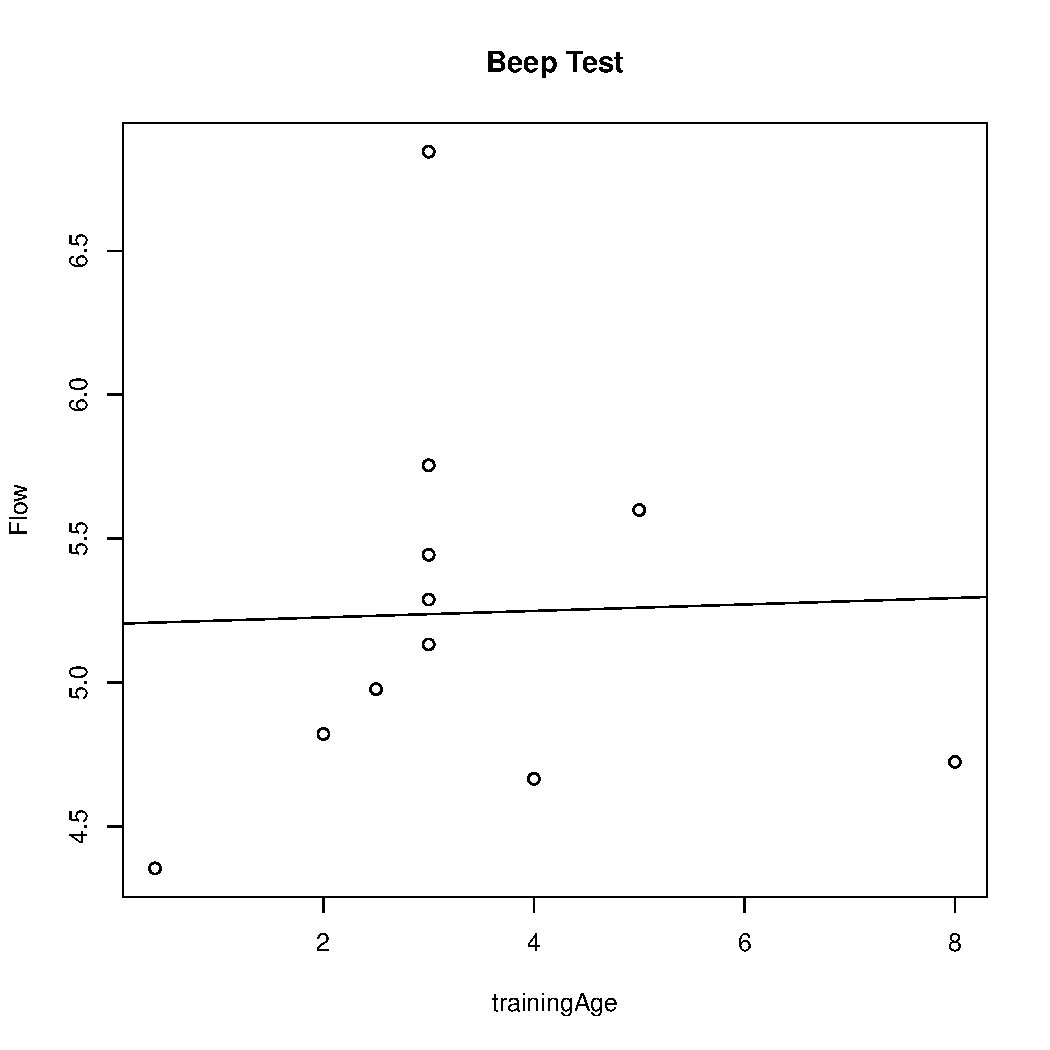
\includegraphics[scale=.5]{images/beepFlowTrainingAge.pdf}
  \caption{Beep Test: Flow State by Training Age (n = 12)}
  \label{fig:beepFlowTrainingAge}
\end{figure}

\begin{figure}[htbp]
  \centering
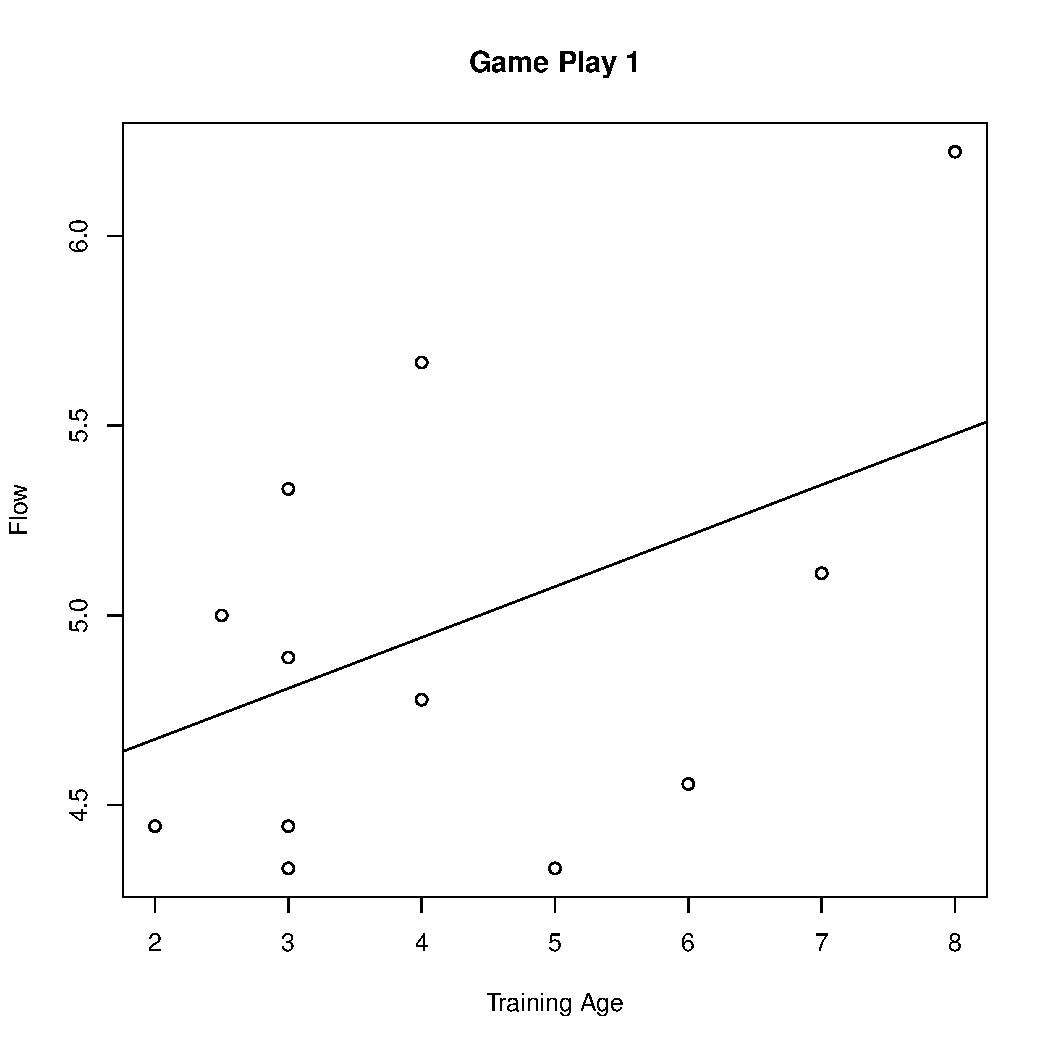
\includegraphics[scale=.5]{images/flow0109TrainingAge.pdf}
  \caption{Training 9th Jan 2016: Flow State by Training Age (n = 16)}
  \label{fig:flow0109TrainingAge}
\end{figure}

\begin{figure}[htbp]
  \centering
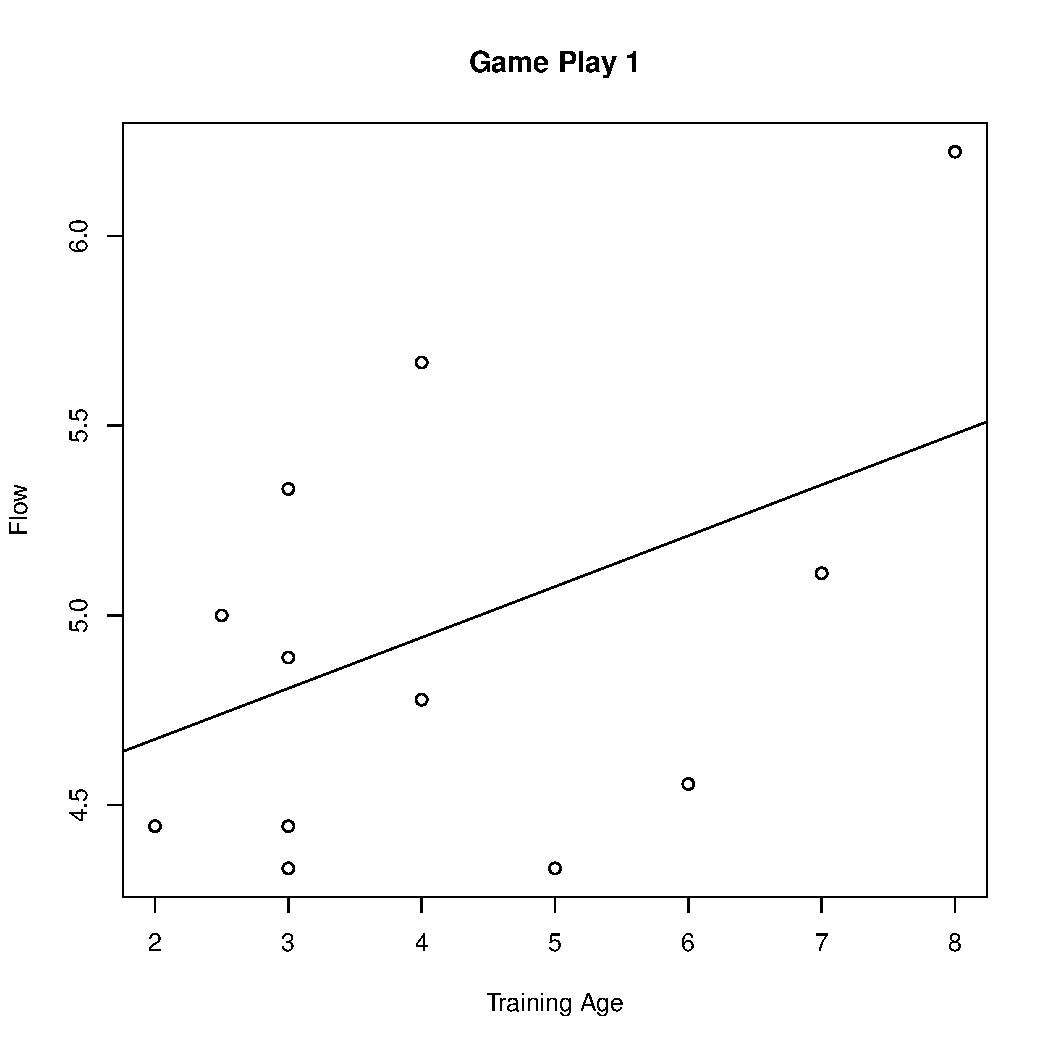
\includegraphics[scale=.5]{images/flow0109TrainingAge.pdf}
  \caption{Training 16th Jan 2016: Flow State by Training Age (n = 16)}
  \label{fig:flow0109TrainingAge}
\end{figure}


\subparagraph{Fear of Criticism}

Athlete responses to two individual items of the flow scale in particular  worthy of further investigation.  Two questions in particular were of relevance:

\begin{quotation}
  Just now I did not care how others would evaluate me
  (刚刚我不关心别人可能会如何评价自己)
\end{quotation}

\begin{quotation}
  Just now I did not care how I performed
  (刚刚我不关心自己的表现如何)
\end{quotation}





\begin{figure}[htbp]
  \centering
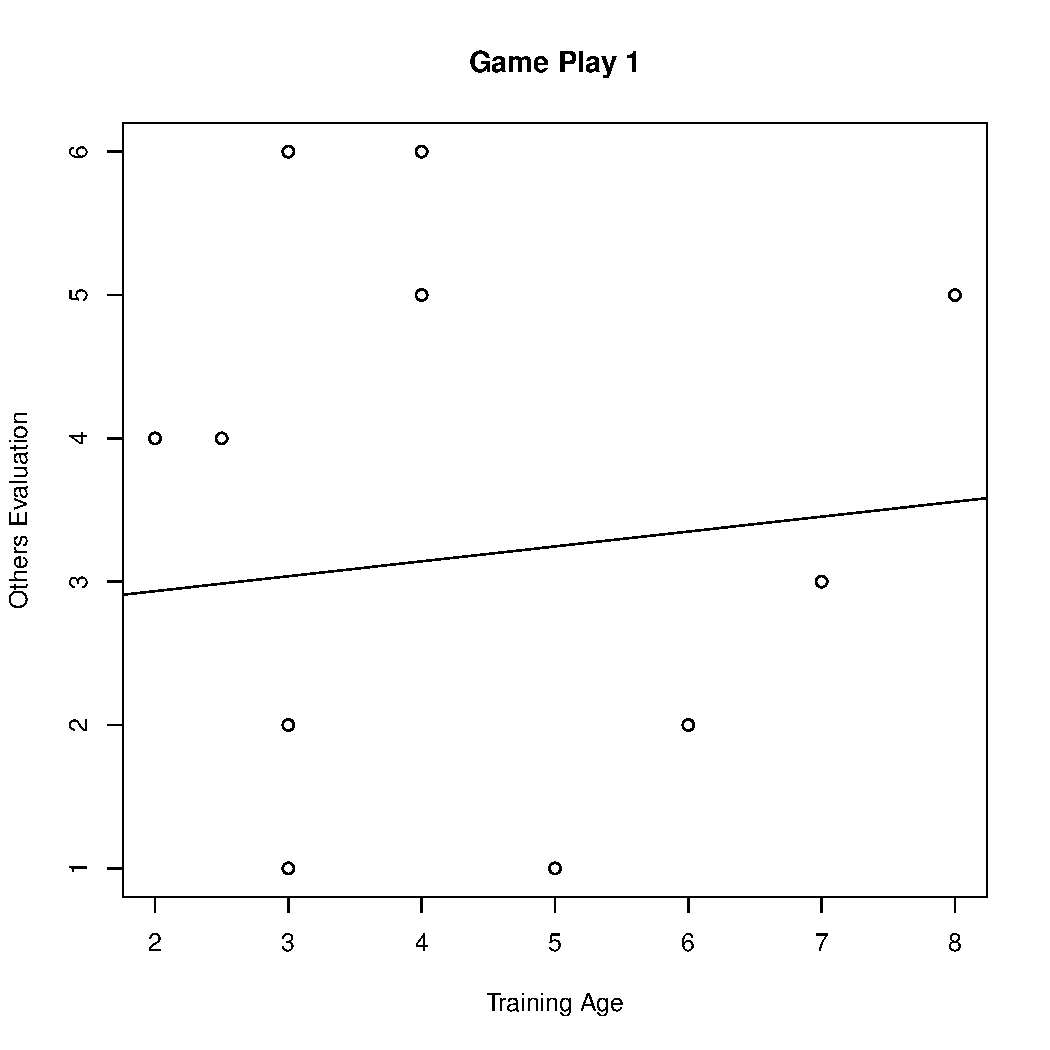
\includegraphics[scale=.5]{images/othersEval0109TrainingAge.pdf}
  \caption{Athletes not concerned by evaluation of others, 9th Jan 2016 (n = 16)}
  \label{fig:othersEval0109TrainingAge}
\end{figure}

\begin{figure}[htbp]
  \centering
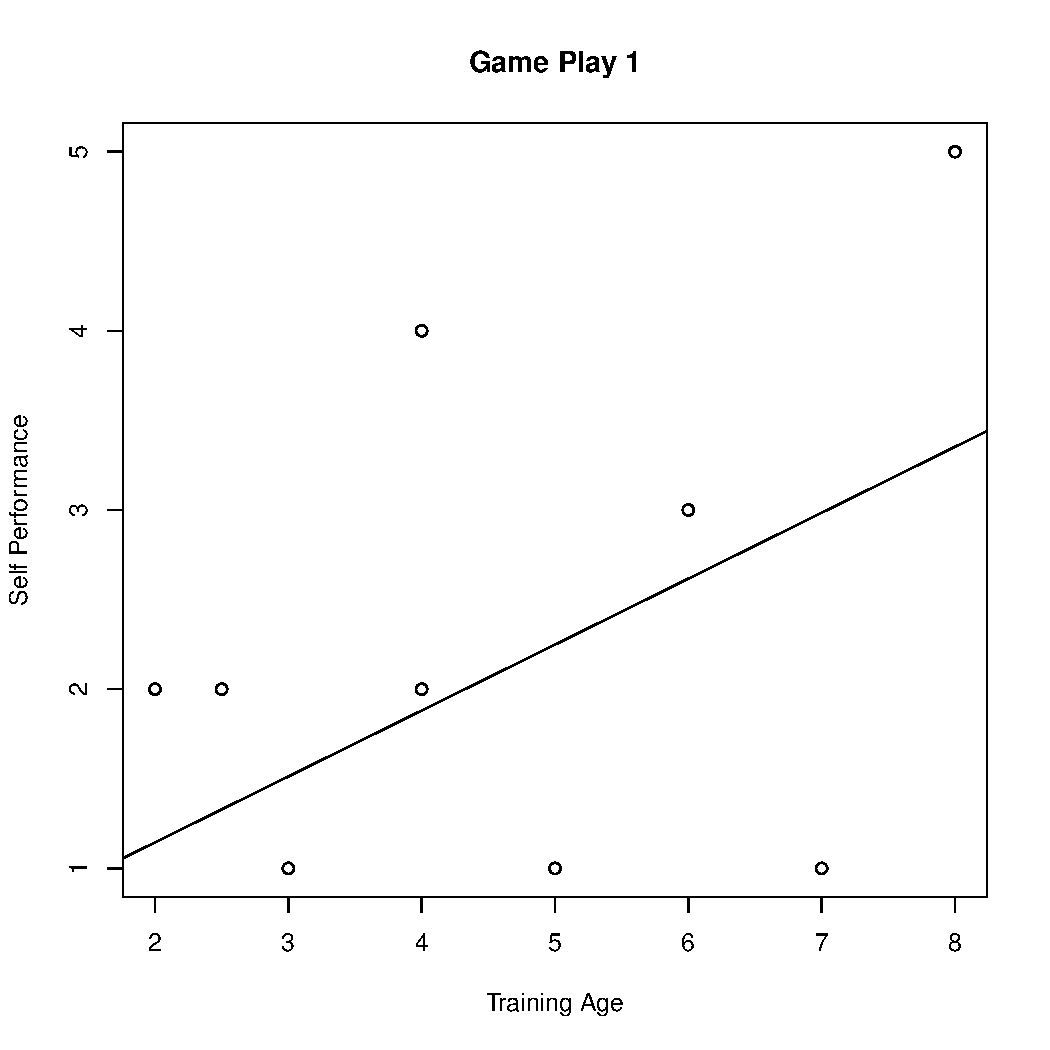
\includegraphics[scale=.5]{images/indPerf0109TrainingAge.pdf}
  \caption{Athletes not concern about own performance, 9th Jan 2016 (n = 16)}
  \label{fig:indPerf0109TrainingAge}
\end{figure}


\begin{figure}[htbp]
  \centering
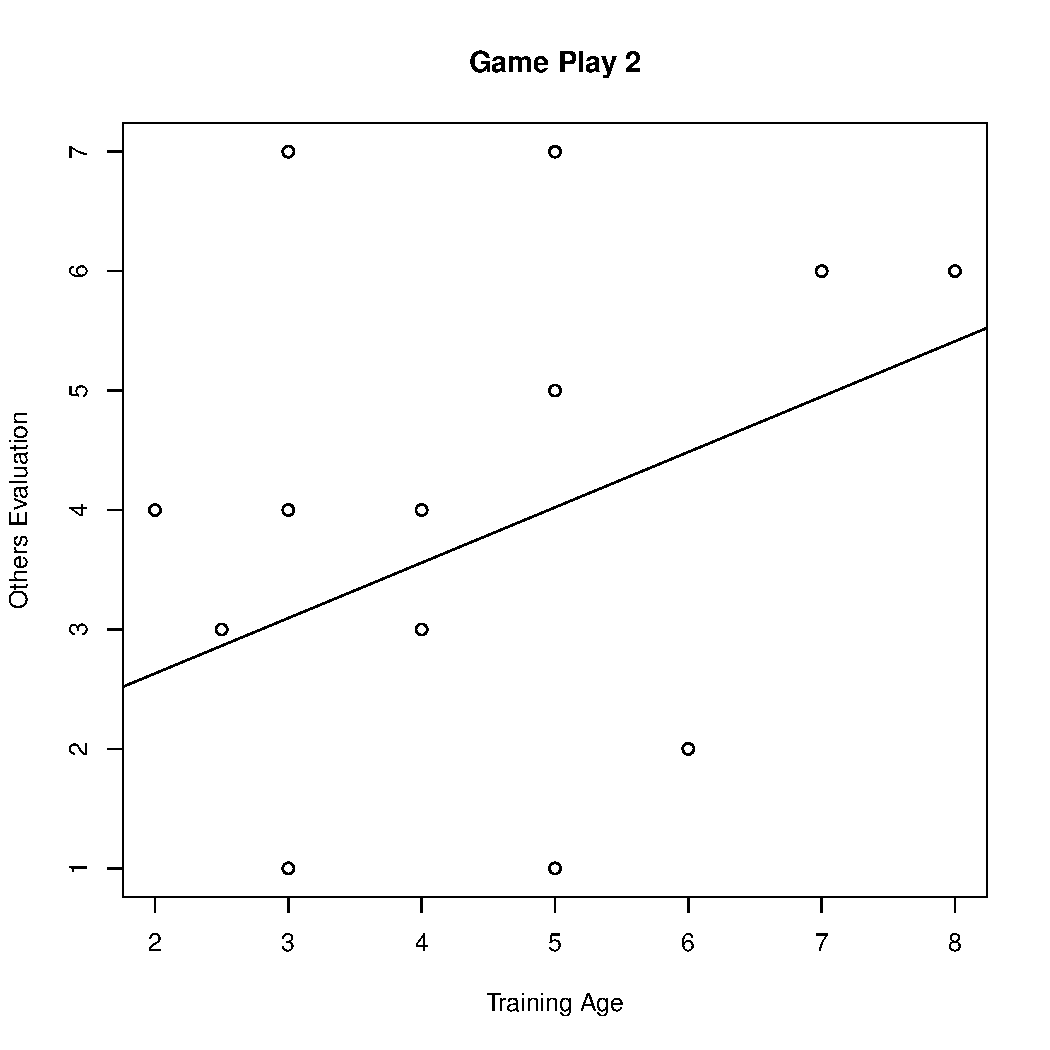
\includegraphics[scale=.5]{images/othersEval0116TrainingAge.pdf}
  \caption{Athletes not concerned by evaluation of others, 16th Jan 2016 (n = 16)}
  \label{fig:othersEval0116TrainingAge}
\end{figure}

\begin{figure}[htbp]
  \centering
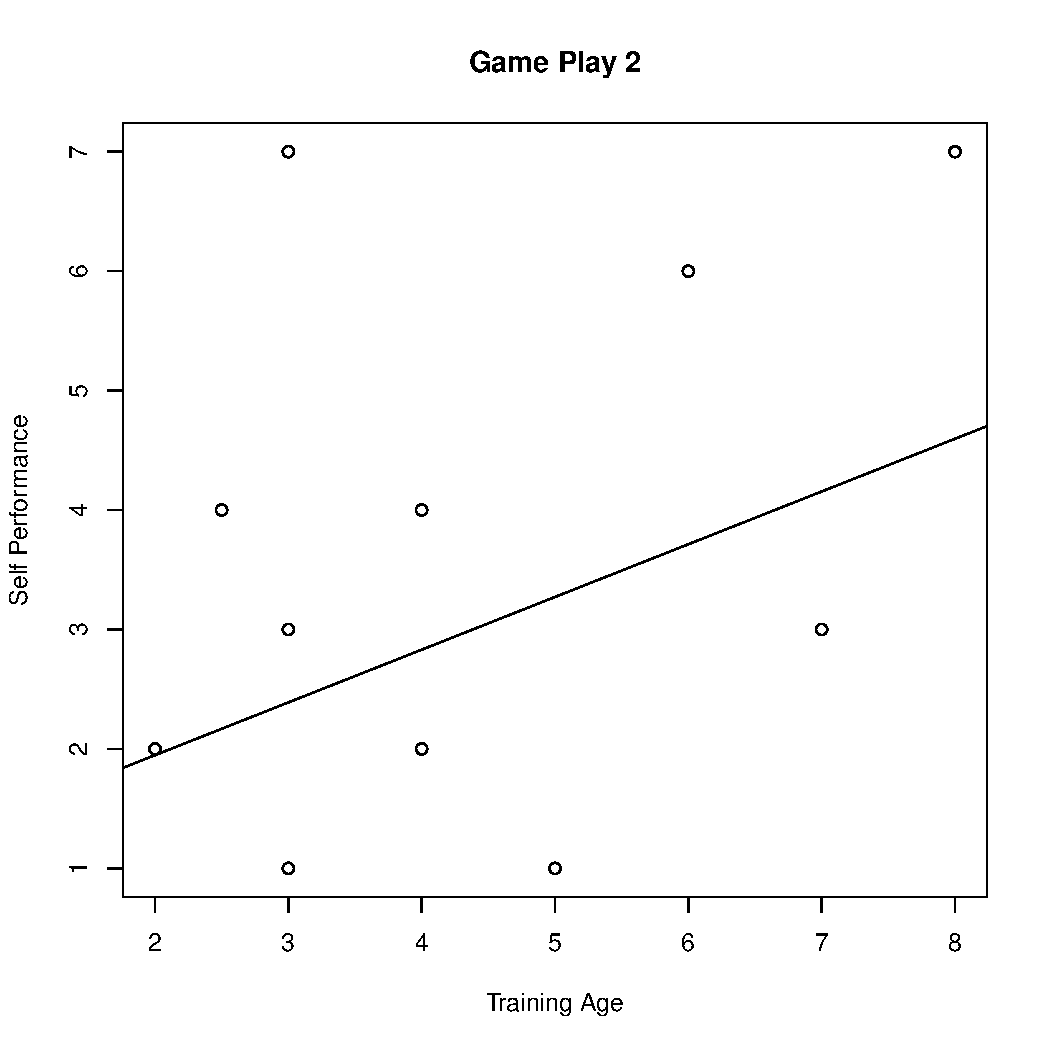
\includegraphics[scale=.5]{images/indPerf0116TrainingAge.pdf}
  \caption{Athletes not concern about own performance, 16th Jan 2016 (n = 16)}
  \label{fig:indPerf0116TrainingAge}
\end{figure}



Comparing the mean scores for junior and senior athletes reveals more  noticeable contrasts.

For the first training session on the 9th January 2016, the overall average score in response to the question ``Just now I did not care how others would evaluate me'' was 3.15(1.95).  The average for senior athletes was 3.67(1.97), while the average for junior athletes was 2.71(1.98).
The overall average score in response to the question ``Just now I did not care how I performed'' was 1.92(1.32).  The average for senior athletes was 2.67(1.63), while the average for junior athletes was 1.29(.49).

For the second training session on the 16th January 2016, the overall average score in response to the question ``Just now I did not care how others would evaluate me'' was 3.67(2.19).  The average for senior athletes was 4.25(2.12), while the average for junior athletes was 3(2.34).
The overall average score in response to the question ``Just now I did not care how I performed'' was 2.9(2.22).  The average for senior athletes was 3.13(2.36), while the average for junior athletes was 2.7(2.21).


\subparagraph{Beep Test and Training: junior athlete comparison}
A comparison of junior athletes' responses to these two questions in the training sessions and after the Beep Test, indicates that the joint action demands of the game play context may be relevant to feelings of anxiety around performance.

For the Beep Test in November 2015, the overall average score in response to the question ``Just now I did not care how others would evaluate me'' was 3.27(1.8).  The average for junior athletes was 2.75(1.75), compared to the averages in the January training sessions of 2.71(1.98) on the 9th January, and 3(2.34) on the 16th January.

The overall average score in response to the question ``Just now I did not care how I performed'' was 3.42(1.16).  The average for junior athletes was 3(1.07).  This average compares to the averages of 1.29(.49) on the 9th January, and 2.7(2.21) on the 16 January.


% othersEvalBeepSeniorAvg 4.305556(1.587956)

%SURVEY RESULTS: relatively equal levels of flow overall, but higher performance related anxiety in junior athletes, particularly in the scratch matches, which required high levels of technical competence and joint action coordination.

%EXPLAIN: perception of performance in relation to social expectations of the team: joint action participation, as well as individual responsibilities (team member, self-determination)

%Senior athletes talk with more composure regarding performance, any deflect responsibility for being the agent of team performance, and show strategy regarding how to regulate energy expenditure.

%IMPORTANT: when compared to the beep test flow survey (with the senior athletes removed), reports suggest that the difference could be related to the technical complexity and scrutiny of coach and senior athletes.

%Bao Yuhan NOSTALGIA for TEAM ATMOSPHERE of the past.  Assumes role of senior, suggests that juniors are too timid, don' talk to senior players, don't let seniors know about anything, worried that senior players will tell the coach.	没有之前那会好了,那会虽然师哥师弟很厉害,但是这个气氛很严重,但是气氛好,现在没有之前气氛那么好了 。现在就是平时在一起师哥师弟很少沟通,师弟也不上我屋来,他们就觉得跟我们老的人在一起聊不下去,没天聊.  人在一起聊不下去,没天聊。有什么事不敢让我们知道,怕我们跟教练说

%Others more generous and circumspect: WW and CSC realise that it's a progression, and that individuals

%EXPLAIN: reduction of dissonance via deflection




\subsubsection{Possible Mechanism: Positive violation of expectations around performance}

The vignette in which I describe Hongwei's journey from timid novice to exhilarated junior team member is designed to pose the question of what mechanism(s) could underpin such a process.  In addition to Hongwei, I noticed evidence of athletes gradually (and at times suddenly) developing a ``feel for the game.''  My discussions with athletes in interviews confirmed the fact that athletes derived considerable motivation from the experience of suddenly discovering that they are capable of performing one aspect of rugby's diverse technical skill set.  Athletes recount with positivity and energy the moment in which their previously held expectations around individual and team performance were positively violated.

Wang Zhengfeng offered one powerful example.  Wang Zhengfeng, now considered a senior athlete, had converted from athletics in 2012, and was an athlete with outstanding physical attributes for rugby---particularly speed and strength. Wang struggled, however, to master some of the basics such as catching and passing and tackling.  I asked Wang about his approach to the challenge of learning the skills of rugby from scratch, and he recounted the time he first discovered that he could execute a side step:

    \begin{quotation}
      JT: How do you overcome this challenge? Do you have a plan or idea? \\
      WZF: I imitate.  Like when I was learning how to sidestep. At the time I’d look at Brother Han (HXL) who had a really good sidestep, I'd just watch him stepping, every day I'd just watch him step, and imitate him.  At the start I probably wasn't practicing it particularly well, I couldn't quite imitate it, but then after some time, I was playing touch and suddenly produced the exact action! I was so happy! Its not like it appeared at a fixed time or anything, it was like suddenly I just moved a step and it happened. And then like after I stepped once I slowly found the feeling, and then stepping became my own thing.  When you pick up new skills for the first time it feels very addictive, I get so happy, when it happens I can stay happy for a long time!
    \end{quotation}

    \begin{quotation}
      JT: 那你自己通过什么样的方式克服这个困难,你有计划和想法吗? \\
      WZF:模仿。就像变相一样,我当时看龙哥做的特别好,我就看他们变向,天天就看哎,模仿一下,可能开始练得不是特别好,模仿不大会,但是时间长了以后,打TOUCH的时候突然做出了这么一个动作!就特开心! 对没有固定的时间出来的,突然动了一步就出来的。比如变向突然出来之后,慢慢就找到感觉了,变相就变成自己的东西了. 做出来新的动作以后就觉得很过瘾,特别开心,能开心很长时间了!
    \end{quotation}

The young hopeful athlete Yang Can, a junior athlete who also had impressive physical attributes for rugby, but was incredibly timid, gave a similar albeit more low key response to a similar discussion in our interview:

    \begin{quotation}
      When I first started practicing, ok, I’ll just carry the ball forward and hit it up (that was all I could do). After that, I discovered that there are many techniques: you can fend people, you can step, you can run into a gap. There are many other actions (than just running straight towards the defence with the ball).
    \end{quotation}

    \begin{quotation}
      刚开始练得时候就是拿着球往前跑,撞呗,后来发现有好多技巧,也可以推人,也可以变向,也可以走空档,有很多其他动作 
    \end{quotation}

While the words on the page perhaps don't quite jump out in the same way that Wang's description does, Yang Can's description of his discovery of rugby's many techniques was a bright and animated spark in an otherwise reserved interview, in which many of his responses rarely involved more than a few sentences.

It appears that the experience of positive violations of expectations around performance can also apply to components of team (as well as individual performance).  As senior player Han explained, he only began to really enjoy rugby when he had an opportunity to coordinate meaningfully with others:

\begin{quotation}
    When I first started training for rugby, when I first started getting exposed to contact I was a little bit afraid, but then after I have been exposed for a longer time I became less and less afraid of contact, and then I felt more and more that as I added a few more things...like when I started to find that coordination between players when playing touch...Because I really enjoy that sort of ``two people coordinating---``pa-pa-pa'' (describing the action of coordinating movement and passes on the field in rugby) passing between players and breaking through the line'' type of feeling, I really enjoy it.
\end{quotation}

\begin{quotation}
  	刚开始练橄榄球的时候,刚接触对抗的时候有点害怕,但是接触的时间长了以后就越来越不怕对抗,后来越来越觉得就加了一些,会打的打TOUCH的时候相互之间有配合,因为我特别享受那种两个人配合怕怕怕配合传球最后突破的这种感觉我特别享受.
\end{quotation}

In a similar vein as both Wang and Yang, Han's animated description of the feeling of ``two people coordinating (pa-pa-pa)'' elicits a positive emotional valence surrounding moments in which expectations around performance are either met or, in the case of an interactional sport of rugby in which expectations are always conditioned by the high uncertainty of the joint action environment, often exceeded.

The fact that both positive and negative violations of expectations around performance featured prominently in both the social and emotional dimensions of athletes' experience of rugby at the Institute suggests the possible existence of an important cognitive mechanism linking joint action to processes of social cohesion.  When expectations around performance are negatively violated, athletes report strong experiences of social guilt (\textit{neijiu}) and rumination on the discrepancy between perceived individual (or team) performance and the expectations around performance that they have internalised from prior experience or authoritative sources such as the coach or more senior athletes.  When these expectations are positively violated, by contrast, athletes show evidence of exhilarated emotional response and agency.  As I will explain in the following section, it appears that when positive violations of performance expectations are specifically located in components of team performance, the result is a range of phenomena possibly relevant to processes of social cohesion.



\clearpage
\subsection{Team Click}
In this section I outline athletes' experience of and attitudes towards coordination in joint action, particularly the phenomenon of optimal coordination, or what I call in this dissertation, team click.  Through my years training and playing with (and coaching) Chinese rugby teams, I knew that there was a specific lexicon for describing optimal coordination in joint action.  The most commonly used term to describe optimal yet effortless coordination is \textit{moqi}(默契), which refers to the phenomenon of `tacit understanding' between two or more people engaged in a joint activity. \textit{Moqi} is a term that applies to all areas of human activity that involves joint action: from sport to music to Chinese comedic ``cross talk'' (\textit{xiang sheng} 相声)---tacit, unspoken understanding between co-actors.  In addition to tacit understanding, I would also hear athletes describe the importance of the ``atmosphere'' (\textit{qifen} 气氛) or ``aura'' (\textit{qichang} 气场) between co-actors or within a team.

The description of these processes, particularly when it derives from personal experience, is particularly animated and emotive, and often appears to contain the experience of positive violation of expectations around performance.  Wang Zhengfeng once again offers an animated description of the phenomenon of team click:

  \begin{quotation}
    It’s really hard for me to say what it feels like.  It feels just like a fight for life or death, like you must win the match.  Normally, that sort of tacit understanding sometimes isn’t there, but then suddenly you coordinate on the field and it you can form this feeling. You haven't given much consideration as to how to play...its probably also to do with the feeling of time spent together, the few of us know each other’s characteristics, we understand each other relatively well.  Its like sidestepping, suddenly you can get that feeling of tacit understanding”
  \end{quotation}

  \begin{quotation}
    还真说不出来是什么感觉。就是感觉生死战一样,必须要拿下来他。那种默契平时有的时候没有,在现场上突然配合就感觉打上来了这种感觉。没有考虑太多怎么打,可能也是时间长的感觉,我们几个知道自己的特点,彼此可能比较了解,跟变相一样,突然就出来了那种默契的感觉 
  \end{quotation}

Senior athlete Wang Wei also offered a rich description of the feeling of tacit understanding and flow in rugby:

  \begin{quotation}
    It feels like the ball in your hand is listening to what you say, it will go wherever you want it to go, whatever you say the ball should do, where it should run, then the ball will go there.  Its the feeling this defender is standing there looking at you and not moving, the whole process goes smoothly (like flowing through clouds or water).
  \end{quotation}

  \begin{quotation}
    	感觉球在手里特别听你的话,你要他去哪就去哪,你说这个球该怎么,该往哪跑,这个球奔哪去。感觉这个防守站在那看着不动。你整个过程行云流水。
  \end{quotation}


When I asked athletes in interviews about the experience of tacit understanding in joint action, I received responses that ranged in the level of detail as well as a level of emotionality attached to descriptions.  As a general rule, more senior athletes were able to produce more granular and detailed descriptions of what they thought were the components of team click with less emotionality attached to these descriptions. More junior athletes, by contrast, tended to produce less detailed descriptions of coordination of joint action, and instead talked about the phenomenon in more general and emotionally charged terms---often, for example, connecting coordination in joint action with ideas of solidarity or unity (\textit{tuanjie} 团结) and cohesion (\textit{ningjuli} 凝聚力) without describing what they thought were the components or causes of the coordination itself.  Alternatively, some junior athletes would acknowledge that they of course knew of the idea of tacit understanding and other components of team click, but that their novice status meant that they had not experienced the phenomenon in rugby in particular, and were therefore unable to comment in any detail.

New arrival Kang Yuzheng, for example, provided a relatively honest reponse to my questioning:

\begin{quotation}
  ZYZ: I have felt tacit understanding before, yes.  The feeling is really good, very flowing. \\
  JT: What is the source of this type of feeling? How do you create it? \\
  KYZ: I haven't thought about it before.
\end{quotation}

\begin{quotation}
  KYZ:有,感觉特别好,很流畅. \\
  JT:这种默契的来源是什么?如何创造?\\
  KYZ:没想过
\end{quotation}


When I asked timid (but slightly more experienced) junior athlete Yang Can if he had ever experienced the feeling of tacit understanding in a team, he responded with the following description:

    \begin{quotation}
      YC: I have before, when I was playing in that National Tournament, in that game against Liaoning Province.  Everyone was giving it their all. \\
      JT: Where do you think this type of feeling comes from? \\
      YC: (This type of commitment) comes from the heart. No matter what, you can’t let the opposition score a try, somehow you must shut them down in defence, and don’t let them run.
    \end{quotation}

    \begin{quotation}
      YC: 有过,在打那个全国比赛的时候。打辽宁那一场,所有人都在拼.\\
      JT: 你觉得这种很拼的感觉来源在哪?\\
      YC: 发自内心的,无论如何不能让对手达阵,怎么样也得死防,一定要防住,不让他们跑.
    \end{quotation}

Yang Can's description is more a description of attitude or motivation for joint action, rather than a description of the components that allow for tacit understanding to emerge.  Ming Xiaokai, one of the unruly undergrads who had been training for a period of time long enough to have experienced at least some variation in the quality of team coordination, offered a slightly more detailed description:

    \begin{quotation}
        MXK: Tacit understanding is definitely there, but its relatively rare. But when you’re up against it in a match you feel very united, especially when sometimes you take the lead again. \\
        JT: What do you think the source of this feeling is?  How do you achieve the result that everyone is working (hard) together? \\
        MXK: No matter whether its on-field things do do with training, or off field things, like some interaction off the field, some communication, when its a bit of fun, when we're all relatively good friends, you know?  When its like this, I feel like I would like to try a bit harder, share more things with others, that type of feeling.  If my teammate gets tackled I'll get really angry and want to help them.
    \end{quotation}

    \begin{quotation}
        MXK: 默契肯定是有的,但是比较少,但是打逆风球的时候会特别团结,有时候会反超. \\
        JT: 你觉得这个感觉的来源是什么?如何才能得到大家一起努力的效果? \\
        MXK: 不光是训练场上的东西,场下的东西,场下的一些交流,一些沟通,比较好玩,比较好朋友吧,我感觉天天场上做的时候感觉想多努力一分,多分享一些东西,这种感觉。他们要是被扑搂了,也会很有气儿,会想去帮助他们。 
    \end{quotation}

Ming Xiaokai emphasises the role of communication and interaction on and off the field in producing the feeling of tacit understanding.  Despite taking the liberty to explore the concept in more detail than Yang Can, Ming Xiaokai also ends up settling on a feeling, in this instance a feeling of solidarity with a teammate.  Lu Zhongsheng (a.k.a. ``Big Mouth Monkey'') was a gregarious senior athlete who was very talkative in our interview.  When I asked him about how to achieve tacit understanding, he replied with much more conviction than his more junior athletes.  His convictions soon led him, however, to drift away from any particular analysis of joint action, and instead towards descriptions of solidarity and emotional closeness with teammates:

    \begin{quotation}
      First of all, you have to have a common direction and goal.  For example, which team are we going to take down today---everyone has this ``must win'' conviction in their mind.  Everyone works together; no abandoning each other and no giving up, most importantly when you’re behind (in a match) you can’t give up, there’s still hope, as long as the time is not up there is still hope.  We shoulder the pressure and are determined to prove ourselves.  It's the presence of that real feeling that ``all for one and one for all''.  And then that feeling of everyone crying together is great! Because we've endured such agony...
    \end{quotation}

    \begin{quotation}
      首先是大家有一个共同的方向和目标,比如说我们今天要把哪个队拿下,大家每个人的脑子都有这个必胜的决心,大家一起努力,不抛弃不放弃,最重要的是及时落后了也不能放弃,我们还有希望,时间还没到我们就还有希望。背负压力,我们一定要做好,就像我们要证明自己。真正的在场上每个人都做到那种“人人为我我为人人”的感觉,然后比完赛大家都一起哭了那种感觉特别棒!很痛苦我们都吃的...
    \end{quotation}


Junior athlete Meng Cheng (a Beijing local and young hopeful from Chaoyang school) provided another powerful interpretation of the components of team click:

      \begin{quotation}
        If we want to play we do it together, and usually there’s nothing we can’t say to each other. For example every week(end) a few of us all drink a bit and eat a bit and chat.  I think this is very important, because if you have a drink and a meal and talk a bit of shit you feel relatively...you generate that feeling you know? Like when you’re drinking together and you feel particularly intimate, really close.  Besides that then its also when you’re doing fitness and can’t keep up and the coach is going to punish you, and so whoever can’t go on you give him a hand and pull him along.  Everyone has the same goal and is motivated.
      \end{quotation}

      \begin{quotation}
        大家要玩一起玩,平时无话不说。比如每周咋们几个大家喝点(酒)吃点聊聊天。我感觉这个很重要,因为你喝点吃点吹点牛感觉是比较。。。你来这个感觉吗?比如说喝的时候感觉特别亲密,特别亲。剩下就是体能训练的时候跟不上教练要罚的时候一起挨罚,谁跑不动了就拉一把。大家目标一致,都有上进心。 
      \end{quotation}


The automatic slippage between talking about tacit understanding in joint action and team solidarity, emotional closeness, and unity indicated to me that, in this context at least, the two constructs were importantly intertwined. Importantly, these observations offer support for theoretical predictions laid out in Chapter 2, namely that a relationship between joint action and social bonding could be mediated by perceptions of performance in joint action---specifically, the phenomenon of team click (HYPERLINK).


\subsubsection{Senior athletes: detail and problematisation}
More senior athletes tended to stick to a more detailed and granular description of what they considered to be the experience of optimal joint action. Interestingly, however, senior athletes would also easily slip off the topic of joint action.  But instead of venturing towards notions of team solidarity and unity, they would instead problematise the lack of these components in the current team, and would point to various rationales for why this was the case.

Old head Cui Shuocheng, for example, reminisced about his feeling of tacit understanding with teammates in Shandong province (before arriving in Beijing):

\begin{quotation}
      When I was in Shandong. Its like when you're moving the ball (passing and catching), when the ball-carrier gets there (indicating to the space in front of us in the interview room) the next person just knows what to do, like he has just one look or something and everything just moves, they both know what to do. I feel that in Beijing (we) play too ``one-out''
\end{quotation}

\begin{quotation}
     	山东的时候有。当你传球和接球的时候下个人就知道做什么,好像一个眼神或者一个什么就动了,知道怎么做。感觉在北京打得太单一,就是传球传球之类的。
\end{quotation}


Senior athlete and coach Lu Peng, always keen to problematise the athletes below him, explained why he thought that the current Beijing team lacked tacit understanding in joint action.  When I asked him if there was any click in the team currently, he replied:

      \begin{quotation}
        No, its very rare.  Not like it was with us before (before 2013), because when we were like that...back then, the status of the Beijing team in China was such that if you were in the starting team for Beijing, it was very hard to experience any disdain.  At that time through our own efforts we would understand that sort of concept from of a ``national team.'' And when we'd go out to compete we'd work hard.  Now they (the more junior Beijing athletes) wouldn't come and find senior athletes to discuss these sorts of things.  They're thinking about their own little things every day.  They won't think about it, and also they won't go and do it.  They skimp their way through training.  It is very important thing for athletes to be--- my former coach used to say this word, I don't know how to say it in English, in China it is that this athlete is has a strong ``animal intelligence.''
        Ok I'll try to explain it to you: animal intelligence is talking about, well first we are all primates right?  And primates are really smart!  So this so called animal intelligence, in the case of rugby, is that on the field you have incredible creativity: you can do things that others don't expect.  This is the idea of animal intelligence in an athlete.  And you can do it often, inconceivable things, extreme intelligence, animal intelligence.
      \end{quotation}

      \begin{quotation}
        没有,很少。不会像以前我们那样。因为我们那样的时候,以前我们北京队在中国的情况下,如果你是主力队员的话,你很难体会含怒。那时候是我们通过自己的努力把国家队的那种理念都看懂了,前后我们出去主要是努力。现在他们不会去跟老的聊这些。天天在想自己的小事情。他不会去想,而且也不会去做。训练的时候敷衍了事。球员很重要一点就是,教练曾经说过一句话,我不知道英文怎么讲,在中国中文讲是这个球员很有灵性! ...我试一下给你解释啊:灵性就是说,咱们单人都是灵长动物是吧?就是特别聪明的!就是所谓的灵性就是对橄榄球的话就是, 在场上你有很好的创造力:别人想不到的你能做出来,就是灵性。 经常能做出来。 想不到的东西,特别聪明,特别灵性.
      \end{quotation}

I went on to probe as to why younger athletes did not display this mysterious animal intelligence in rugby:

\begin{quotation}
      JT: Why do you think the young athletes don't have this intelligence, is it because they're not motivated? \\
      LP: That's right, its a problem with the environment they're in, there is no competitiveness, no motivation.  At that time we were very competitive and so we were motivated.
\end{quotation}

\begin{quotation}
      JT: 那你觉得年轻队员不做这个是因为没动力?\\
      LP: 对,环境问题嘛、没有竞争力,没有动力。我们那时候就是很有竞争力,有动力。
\end{quotation}

The two components of Lu's nostalgic monologue that are worthy of attention are: 1) the way in which Lu employs the opaque concept of animal intelligence to describe optimal joint action in rugby, and 2) the way in which Lu locates the reason for a lack of on field click in the current team in the lack of competition and motivation among the junior athletes.  Both of these components indicate that Lu lacks direct access to the mechanisms of joint action, but nonetheless is in a position of authority from which he is able to perform elaborate exegesis on the state and quality of team coordination.

Senior athlete Ma Haitao explained Beijing's issues with coordination in joint action as a cultural issue:

\begin{quotation}
  MHT: Chinese people's sense of initiative is very poor.\\
  JT: Why do you think its like this, really? What is the reason? \\ MHT: Environmental factors, environmental influence.  Like you all (Westerners) from a young age in your environment you think its just has to be done like this.  Our environment isn’t like that.  First, (in a group situation) you will think ``we are all teammates,'' and your team all think that this principle is very important.  But we all think ``it doesn’t matter, I can just go with the flow and that’s enough.''  But you are not like that, you are like ``this is just how it must be done.'' Just like what we were talking about in the gym, about your personal ``disposition'': you said you need to get up in the morning and feel like you're being productive... China also has this disposition, its always ``have a look first'' (before committing to anything)...
\end{quotation}

\begin{quotation}
  MHT: 我们中国人自觉性很差. \\
  JT: 为什么?到底?原因在哪?\\
  MHT: 环境因素,环境影响。像你们,从小你们环境影响觉得就该是这样。我们环境影响不是这样。一是认为``你们是队友'',你们队都觉得这个很重要!但是我们觉得 ``无所谓,我变通一下就可以了''. 但是你们就不是,你们是 ``他就应该是这样了''就像我们在健身房聊天说那个 ``形势'', 早上起来要干啥,中国也有一口, 他就是总的形势是  ``看一下'',他不会...
\end{quotation}


Senior athlete Pan Qiyu also critiqued the Chinese system, drawing attention to the fact that the Chinese competitive sport system is inherently problematic for fostering effective on field coordination:

\begin{quotation}
  I think you take Chinese football, if you’re talking about competitive sport system in China, the Chinese football team can barely beat a random student team, everyday is a battlefield (warfare)! There’s no thinking in competitive sport, nothing in the brain, no innovation (to use a foreign way of speaking), there is no will to build emotional connection, coordination, or tacit understanding (click) between teammates, and so it leads to this type of feeling at the moment.  So that's why I think Basketball, football, rugby must all develop via as school sports, like America, Japan and also Europe, the’ve all developed their sports in schools, from a young age, first they develop interpersonal skills of communication and team awareness, and I think this is really great.  The Chinese sport system is missing this.
\end{quotation}

\begin{quotation}
  我觉得这个中国足球,竞技体育,连个学生把子都踢不过,天天战乱!,所以竞技体育,人的脑袋没有东西,没有创造力(就是用外国的说法),队员之前没有感情,没有配合,没有默契的意志,导致这种感觉。所以我还是觉得什么篮球,足球,橄榄球必须走校园体育开展。应该像美国日本包括欧洲,都是在校园开始开展,从小开展,一是培养人与人之间的沟通和团队意识,我觉得这个比较好。中国体育体制就却这个
\end{quotation}

When I then went on to ask Pan about the feeling of tacit understanding and team click, he naturally drew upon his critique of what was lacking in the Chinese sports system to describe what is important to optimal coordination:


\begin{quotation}
  PQY: I have experienced the feeling of tacit understanding, yes. I've had harmonious times and unharmonious times. When I was in Dandong (Liaoning Province) that team was relatively harmonious.  The seven of us on the field I felt were pretty unified, I felt that that kind of atmosphere was really good. \\
  JT: What do you think is the source of that feeling? \\
  PQY: Every individual is inclusive and positive, and accommodating of each other. Every individual has weaknesses, but then everyone is accommodating of the weaknesses on the field, I feel that its better like that, its more motivating, it makes people...
\end{quotation}

\begin{quotation}
  PQY:有过,有过和谐的时候也有不和谐的时候,我在丹东的时候那支团队比较和谐,我们场上的那七个人我感觉是比较团结,感觉那种氛围感觉比较好 \\
  JT: 你觉得这种感觉的来源是什么?\\
  PQY: 每个人很包容和积极,大家都很互相包容。 每个人都有缺点,但是每个人都包容每个人的缺点在场上, 我感觉这个比较好,比较动力,比较能让人。。。
\end{quotation}






\clearpage
\subsection{Group Membership (Social Bonding)}

Athletes' descriptions of components of team click reveal that questions framed in terms of on field coordination can easily drift into reflections about the broader social processes and dynamics of the team.  The extracts included above offer evidence of a relationship between the phenomenon of team click and processes of group formation and perhaps, ultimately, social cohesion. It was clear from my ethnographic observations that despite the utilitarian motivations of individuals, coaches, and officials, the rugby program at the Institute provided offered rich psychological resources.  Athletes clearly found friendship, emotional support, guidance, and, importantly, identity by virtue of their membership to the team.  Lian Jianxiang, a young trialist of the Coach Zhu era of the team left the team in February 2016, shortly after Zhu left.  Nonetheless, even though all of the utilitarian benefits that adherence to the program offered had all but disappeared for Lian, in August 2017 I ran into Lian on the sidelines of the National Games in Tianjin. Lian was in Tianjin to support the Beijing men's and women's teams.  He wore his Beijing Team apparel and banged loudly on the supporter drum all weekend in support of his former team.

When I asked athletes to expand on their thoughts around group membership, three core categories emerged.  Athletes tended talked about the following components being important to their connection to the team 1) emotional support derived from group membership, 2) a sense of a common goal, and 3) social identity. I will review ethnographic evidence under each of these categories.


  \subsubsection{Emotional Support}

As interview data suggest, some athletes describe the feeling a strong emotional connection to their teammates and to the team.  As Meng Cheng explained: ``you generate that feeling you know? ...you feel particularly intimate, really close.'' Lu Zhongsheng recounted a similar phenomenon: ``It's the presence of that real feeling that `all for one and one for all'.  And then that feeling of everyone crying together is great! Because we've endured such agony...''   Even the intense critiques of the state of the team launched by the likes of Lu Peng and others are in their own way an indication of emotional attachment to the team; a less invested individual would conceivably not spend the time and energy on such exegesis.

As junior athlete Yang Can explained when I asked him about his experience of group membership:

    \begin{quotation}
      Because rugby is a team sport, you know. We’re all brothers, it's the same as fighting, we’re born brothers and we’ll die as brothers you know, like a family, all together, thinking about how to share the responsibility. Its really good...I had never experienced this feeling before.  At that time at primary school there weren’t any rules, you’d just muck around or at the end of school just leave straight away, there wasn’t this type of feeling there.
    \end{quotation}

    \begin{quotation}
      因为橄榄球就是团体项目嘛,都是兄弟,像打架一样,出生入死得兄弟嘛,就跟一家人一样,互相,多替别人考虑分担,挺好的...没有过这种感觉,那时候小学没有什么规矩的,直接玩或者放学就大直接走了走了,没这种感觉
    \end{quotation}

At the time that I interviewed him, Guo Junping  was one of the team's newest trialists, from Fujian province in China's south.  Zhu had organised for Guo to come to Beijing after a recent scouting trip to Fujian.  Guo had just finished high school, and was no doubt interested in opportunities to attend university. he had never played rugby before, and had only a brief background in athletics before arriving.  When I asked him about his views on rugby, after only a few weeks of training in Beijing, he responded:

  \begin{quotation}
      I really like this sport.  I liked it at the time that Huang introduced it to me (his coach in Fujian). Its unlike athletics, athletics is an individual sport, I prefer teams.  There is more passion, there are mates playing together.  Its like playing computer games, I’m happy when there are people to play together with, it's a team sport.
  \end{quotation}

  \begin{quotation}
    	挺喜欢这个项目。当时黄老师介绍时候我就喜欢,跟田径不一样,田径是单人项目,我比较喜欢团队,比较有激情,有伙伴一起玩,跟玩游戏一样,有人跟你一起玩就开心,团体项目。
  \end{quotation}

Computer games were extremely popular among the athletes, both junior and senior.  At the time, from what I could gather by way of conversations, the most popular came among the athletes was a game called League of Legends.  League of Legends (LOL) is a is a multiplayer online battle arena video game, in which small teams of individuals team up to fight other teams.  Many meals that I attended with the team at the canteen were dominated by discussions of computer games, specifically LOL. I was usually a passive listener in these conversations, but sometimes involved myself in an attempt to learn more.


``Actually,'' said Lu Zhongsheng, turning to me, ``there are so many similarities between LOL and rugby. So its no wonder that we love playing them.  Different characters have different strengths, 1on1 battles are the basis, but then it also relies on team work and team formations and strategy.''  Lu's comments were consistent with some of the research conducted by Hornbeck on gamers in China, which suggests that explanations for gaming should not be limited to the fact that they promote competitive and violent behavioural tendencies, but that they also provide a space for the activation of moral cognition, one dimension of which includes belonging to a supportive (virtual) community. Han continued the conversation:

    \begin{quotation}
          The thing with gaming is that there are such low entry costs - you might not be that good, but at least anyone can play (he motioned the clicking of a computer mouse with his thumb, index and middle fingers).  Sport isn’t the same, if you can’t run or pass or kick then there’s no way you can participate.
    \end{quotation}

This led Wang Wei to start talking about a gamer who only has one arm, and so uses his leg and foot to control the keyboard, and his arm to control the mouse.  Everyone laughed but also expressed respect and wonderment. It served as a conclusion to the conversation that online games are in fact a huge phenomenon.  This conversation helped explain the reason why Guo Junping chose to use computer games as an analogue for rugby.  The sense of team, and of belonging to a team appear to be a core reason for the comparison.

Pan Qiyu, a senior athlete and CAU graduate student was ever-eloquent in his articulation of the emotional support of the group in rugby:

    \begin{quotation}
      I think that through rugby you can meet friends, you can train your awareness of social unity, and this sort of awareness of hard work, toughness, and struggle. I think all these things are very…for example every time you run fitness, at the time it is incredibly tough, but once you’ve finished your mood is extremely cheerful, even though you are very exhausted, its still really happy.
    \end{quotation}

    \begin{quotation}
      我觉得通过橄榄球能交朋友,能锻炼自己的团结的这种意识,刻苦,艰苦,奋斗的这种意识,我觉得这些都很。。。比如说每次跑体能啊,当时特别辛苦,跑完之后心情非常愉快,虽然跑得很累,但是跑下去很愉快的感觉。 
    \end{quotation}

Similarly, unruly undergrad Ming Xiaokai expressed his experience of team membership:

    \begin{quotation}
      Friendship: the feeling of playing alongside really good friends, good mates, scoring a try together, winning by one score after the scores are level all game, its especially, especially joyous, very exciting.  That's it really, when things are really tough, and when we all come in and put our hands on the ball, I’m really happy.
    \end{quotation}

    \begin{quotation}
       友情。和特别特别好的朋友,特别特别好的哥们儿,一起打球的感觉,一起达阵,平分赢一个球一起赢的那种激动,特别特别开心,很激动。主要就这些,特别困难的时候,打发成球,特别开心.
    \end{quotation}


These interview excerpts are strong indicators that processes of group membership associated with the rugby team at the Institute offer athletes a level of emotional support.



\subsubsection{Common Goal}

Another recurrent theme in interviews was the impression of team members sharing a common goal.  As Meng Cheng explained when describing that ideal team feeling, ``everyone has the same goal and is motivated'' (大家目标一致,都有上进心). Vice-Principal Jenny also pronounced the importance of unity around a shared goal in her official address to the team, back in November 2015.  ``I don't wish to see...[you] take the field with seven hearts, or five hearts...I wish to see that everyone shares only one heart'' (我不希望大家...上场之后七条心、五条心...只希望大家一条心).

Wang Zhankun, a junior athlete and young hopeful of Chaoyang school, provided the following response when I asked him what he had learned from transitioning from an individual sport to a team sport:

  \begin{quotation}
    Unity, seven people bound together, not like in an individual sport, where you’re just one person, in a team sport you must have seven people with one heart you know, play against them with one heart.  If you have one who is not on board then you’re whole team is no good. Individual sports detract from feeling of belonging: if you’re going ok its ok, but when you’re not going ok its like ``this is bad, that is bad''.
  \end{quotation}

  \begin{quotation}
    团结,七个人绑在一块,不像个人项目,就自己一个人,团体就必须得七个人同心嘛,同心和他们打。有一个不同心你整个不行 (2) :没有,还分神呢,好的时候不要想,不好的时候: ``这个不行,那个不行''
  \end{quotation}

  Han also offered a similar description when I asked him whether or not athletes were motivated to work for their teammates. In this instance, Han emphasised that shared goal does not necessarily shared roles, and instead division of labour and knowing one's place in the team is important in the achievement of a common goal.

    \begin{quotation}
        Oh, sometimes I feel that there is such a feeling, that we are all a team, I do my job, you do your job, and everyone is developing towards a common goal.  Because in China its like this, when our team’s results are good, every person in our team benefits.  Everyone must work their way up together, progress together, for us to be better. I have this awareness.
    \end{quotation}

  \begin{quotation}
      	哦,我有时候会有会有这么一个感觉就是,我们大家是一个团队,我做好我的,你做好你的,大家都往一个共同的目标发展,因为我们中国是这样,我们球队的成绩好的时候,我们球队的每个人都会收益整。大家都要相互往上走,相互进步,我们才会更好。我有这种意识。 
  \end{quotation}

These excerpts emphasise the idea that all team members are working in the same direction. The idea of a shared goal is related to the way in which key members of the team insisted to me that the coordination of the entire system is important for the team to be effective (see Chapter 5, Section X HYPERLINK).




\subsubsection{Social Identity}

In addition to emotional support, and the perception of a common goal, it is clear that athletes also derive resources for social identity formation from group membership.    As discussed in the previous chapter, the dominance of hierarchical relationism means that athletes explicitly understand their social identity as interdependent with the social identity of others.  In contrast to a conception of social identity theory, in which the individual understands group membership as a function of psychological distance between the category of self and the category of group, hierarchical relationism starts from the default position that all group members are already fused to a highly distributed group identity, and social resources are acquired through a fostering of hierarchical relationships within the group.  For the Beijing team, the team is more nuclear family than it is an egalitarian forum for diverse independent interests.  This group, regardless of its specific structure, provides athletes with resources to generate a social identity.

Social media was a highly visible forum in which athletes would signal their social identity.  Athletes junior and senior would display their connection to rugby on their individual WeChat accounts, by either changing their alias to include some reference to ``rugby'' or their profile picture, to display a photo of a rugby ball or a famous rugby player (see Appendix HYPERLINK).  Athletes commented to me that the rugby team at the Institute used to be the most formidable and successful team in the Institute, and that despite the recent fall from grace, the rugby team were still highly revered by the rest of the athletes at the Institute.

Among the 26 athletes I analysed, I observed variation in the intensity of identification with rugby.  As the various factions in the team indicated, there was a range of positions that athletes occupied, ranging from the newest arrivals, through to the handful of athletes who had been at the institute for five years, and some of those athletes (Han, Lu, and Su Hailiang) had been training for rugby prior to 2010 at CAU.

I observed three general categories of social identity drawn from involvement in the team: 1) the newest arrivals and athletes below university level tended to express their interest and like of rugby and enjoyment of the team environment, 2) the unruly undergrads described varying levels of attachment to rugby and the social identity that it afforded, and 3) senior athletes described complete alignment with rugby, such as their identity and future career path aligned with rugby in such a way that, as Han expressed to me, they ``just want to do this (rugby)'' (就想干这个).
      %Fun/interesting/compelling (juniors)

Yang Can, a young hopeful from Chaoyang School, summed up the way in which many new arrivals described their identification with rugby:

      \begin{quotation}
        I like it, because when I first tried it I thought it was really enjoyable...for example, the ball is oval shaped, you can pick the ball up and run with it, you can pass it, fend people and whatever.  Its very...very...very fun.
      \end{quotation}

      \begin{quotation}
        喜欢,应为刚开始的时候觉得挺好玩的.	比如球是椭圆的,拿着球可以跑,可以传啊,推人什么的,挺。。。挺。。。挺好玩的 
      \end{quotation}

Kang Yuzheng offered a similar albeit more reserved recognition of rugby and his level of enjoyment.  I had to more actively draw out his response:

      \begin{quotation}
        JT: Before you arrived at the Institute did you know about rugby?\\
        KYZ: I had played touch rugby for half a year at school...Yeah, I thought it was really enjoyable.
      \end{quotation}

      \begin{quotation}
        JT: 来先农坛之前知道橄榄球吗?\\
        KYZ: 我跟学校练触式橄榄球练了半年...恩,感觉还挺好玩的
      \end{quotation}


\subparagraph{Enjoyment yoked together with education}
The theme of enjoyment of rugby was a recurrent theme when asking athletes about their motivations for adherence to the sport.  Many athletes would cite the obvious incentive of pursuing rugby for the opportunities for tertiary education that it provided.  But this rationale would often be yoked with the idea that enjoyment was a similarly motivating factor.  As Lu Explained:

    \begin{quotation}
      At the time I stayed here (to play rugby) for two reasons.  The first was that I thought this sport was really enjoyable. The second was also rather precise, one really important thing that came to me was that coach Zheng Hongjun assured me that he would solve my schooling problem, and so then I decided to stay here.
    \end{quotation}

    \begin{quotation}
      当时留下来有两方面的原因,第一是我觉得这个东西很好玩。第二也是算很确切的,很重要的一个东西涌向我就是,郑教练给我保证说会给我解决上学的问题,然后就决定呆在这里了。 
    \end{quotation}

Ming Xiaokai offered a similar rationale, citing education first, and enjoyment of the sport as a secondary motivation.  When I asked him what his parents thought of him playing rugby, he explained:

    \begin{quotation}
      They (my parents) don't have many thoughts about it, because they think me making it in to university is already fantastic! I am now already at university (at BSU), but I play this (rugby) because I really like it, I still want to keep developing with it. Before it was for getting in to university, after making it to university now I want to train hard, now I really want to develop this thing.  Before it was all for getting into university, now that I'm at university I think its really good, I can't let go of it.
    \end{quotation}

    \begin{quotation}
      他们没有什么太大的想法。因为他们想我考上大学已经不错了!我现在已经上大学了(体大),但是我是喜欢这个东西才还练,我还希望在往上走一走...之前为了上大学,上大学之后就想好好练,现在就想好好发展这个东西。之前是为了上大学,上大学以后的感觉挺好的,放不下.
    \end{quotation}

Lian Jianxiang also felt compelled to yoke enjoyment to his rationale about pursuing rugby for the pruposes of education:

    \begin{quotation}
        Before I wanted to go to university there (at my old school), but I didn't get in.  Then I heard there was this program here, I really liked rugby, but my province didn't have this sport. At the time my coach said that there was this opportunity, if you play rugby you'll be able to get into university.  And so I wanted to come and give it a try, and as a result I've been here until now.  I really like (rugby).
    \end{quotation}

    \begin{quotation}
        我之前在那想考学,但没考上。后来听说有这个项目,我挺喜欢这个项目的,但是我们当时省里没有这个项目。当时(教练)说这有个机会,练橄榄球就有机会上学。我就想来试试,结果就一直到现在。挺喜欢.
    \end{quotation}

I am not suggesting that the inclusion of enjoyment as a rationale for adherence to rugby was a strategy employed deliberately by these athletes to disguise the utilitarian motivations behind their interest in rugby at the Institute.  These rationales do, however,  communicate the social resources that the program provides to athletes.  All athletes in the program were completely immersed in the life of the team, by definition of their identity as team members.

The trajectory of athletes in the program, ranging from new arrivals to young hopefuls to undergraduates to senior athletes, displayed a progression of social identity that progressed from enjoyment to more substantial and irreversible processes of social and psychological attachment.  Ask Ming Xiaokai continued to explain to me (following on from his comments immediately above):

\begin{quotation}
    I only learnt about rugby after I came to XNT, before I was training for athletics. I have been training for just on two years now, before that 100m track.  Right at the start I found it hard to accept, I didn’t really like it. Now I think I already have that feeling where I can’t leave.  I’ve now had that time to understand it, I now like this sport, but I’m still really really poor at it
\end{quotation}

\begin{quotation}
    我是来先农坛之后认识橄榄球的,我之前是练田径的。打橄榄球刚两年,之前是百米田径。刚开始很难接受,不太喜欢,现在觉得已经有点离不开的感觉了。有了这个理解的时间,喜欢这个项目,但是练得还是差很多很多.
\end{quotation}

As Lu Zhongsheng explained in his reflections to me (included above), the feeling that one ``can't leave'' is in one sense the product of other possible doors closing for athletes as they become more and more invested in rugby.  But on another level, the attachment that Ming Xiaokai describes is also a psychological attachment to rugby and the team as the source of belonging and social identity formation.

Ma Haitao explained to me the development of his feelings of belonging to the team:

  \begin{quotation}
    When I first came my sense of belonging was not strong, in terms of joining the Beijing team, because I didn’t have anything, I couldn’t play! I wasn’t playing with the team, I wasn’t anything.  At the time in my heart I felt, being a Beijing Team member means going out and representing Beijing in a tournament.  If you haven’t represented Beijing then I felt like I hadn’t made a contribution, I could say to myself that I was part of the team, but I couldn’t actually recognise myself as Beijing team.  Now, last year when I played in a tournament, now I have that recognition. ``Are you in the Beijing team? Have you played in a tournament?'' (If the answer to these questions is) no, then I don’t acknowledge myself.  Only last year after playing a Tournament did I slowly start recognising that I was part of Beijing team.
  \end{quotation}

  \begin{quotation}
    刚来的时候归属感不强,就加入北京队,因为什么都没有,啥都不会,没跟着一块打球,什么都不是。当时心里觉得什么是北京队,就是出去代表北京队比赛。没代表北京队就感觉自己也没为北京队做过贡献,说自己是北京队,自己都不认可自己是北京的。现在去年打比赛了,才对自己有认可。“你是北京队么?比过赛么?”没有。自己不认可。去年打完比赛才慢慢开始自己认可.
  \end{quotation}

Ma explains that his ability to equate his personal identity with that of the Beijing team was contingent on him representing Beijing in national tournaments---before doing so he ``was nothing.''  This passage is a great demonstration of the power of the group as a coordinator and administrator of social identity.  It is interesting to note that for Ma, concrete on-field actions (taking the field for Beijing) signal authentic group membership.

Senior athlete Wang Wei explains that his identification with rugby was a gradual process of familiarisation. Once familiarised, however, Wang came to like the sport, in a permanent, irreversible sense:

  \begin{quotation}
    I guess its exposure, when I first started my first impression was that it was barbaric, then after that slowly after more exposure to rugby I thought that this sport is really suited to males, I thought that this sport is a really good sport, I thought I had gradually come to like this sport.  At the beginning I thought it was too barbaric and wasn’t game to play, not game to tackle anyone to the ground or whatever, but after I’d been exposed to it for a long time, I came to understand the culture, and I came to like the sport.
  \end{quotation}

  \begin{quotation}
    还是接触吧,刚开始第一印象觉得野蛮,后来慢慢接触之后觉得这个项目挺适合男性运动,觉得这项目是个挺好的项目,觉得自己后来慢慢喜欢这个项目了。开始的时候觉得野蛮不敢打,不敢扑倒什么的,后来接触的时间长,了解这个文化了,就喜欢上这个东西了.
  \end{quotation}


Han was perhaps the most adamant of his 1:1 fusion with rugby.  Han was the most experienced athlete and was also in a position in which he was uncertain about his future, but certain that the only skills he had to face the future were associated with rugby.  As he said to me when I first arrived at the Institute and, not knowing the details of the politics of the situation, asked him what he was going to do next after the 2017 National Games.  Han smiled at me, recognising that at that time I had no idea about the details of his situation with the Leadership of the Institute. ``I don't know yet'' Han said to me, ``But all I know is that I just want to do this (rugby).''

Later in our semi-structured interview, Han explained his relationship to rugby in more detail:

    \begin{quotation}
      HXL: I think its like this: as long as I like something, then I’m willing to pay.  And then I might get injured, or let myself get tired and fatigued or whatever, but I think ``I really like this sport, I am willing to do it.''\\
      JT: And once you come to like (rugby), these costs don't count as...\\
      HXL: Once you come to like rugby you're willing to invest a lot in it
    \end{quotation}

    \begin{quotation}
      HXL: 我觉得是这样,只要我喜欢这个东西,我就愿意去付出,然后可能会受伤啊、或者让自己很累很疲惫什么的,但是我觉得我挺喜欢这个项目,我愿意去做。\\
      JT: 喜欢了之后,这些成本不算...\\
      HXL: 喜欢之后可以付出很多.
    \end{quotation}



\myparagraph{Rugby as a space for self-validation}

In addition to explicit examples of social identification mentioned above, I also noticed that group membership in rugby offered athletes a space in which they are able verify and validation individual identity.  As Fang Chao said to me in our interview, the social demands of rugby had transformed him into a ``completely different person'' (觉得我完全不是同一个人了).

Yang Can, for example, professed proudly to me that rugby had allowed him to learn a lot of things:

\begin{quotation}
    I have learnt that you have to keep moving forward with every step, you can’t move backwards, you have to have an awareness of moving forward.  Also, when defending you absolutely cannot let your opponents advance forward.
\end{quotation}

\begin{quotation}
    学会了每一步都要向前,不要往后退,要有向前的意识。还有防守的时候绝对不能让对手前进一步
\end{quotation}

Although Yang Can was technically referring to on-field concepts, he spoke about them in a way that clearly signalled that he was talking about off-field virtues for self conduct.

Ming Xiaokai offered a similar rational for his adherence to rugby: it served as an opportunity to prove himself:

  \begin{quotation}
    Not I feel the main motivation is to prove myself, show the current coach, because I think the current coach doesn't really acknowledge me, so my biggest goal is to make him acknowledge me.
  \end{quotation}

  \begin{quotation}
    现在我感觉主要的动力就是想证明自己,给现在的教练看,因为我觉得现在的教练对我不太认可,所以我现在最大的目标就是想让他们认可我
  \end{quotation}




Senior athlete Lu Peng, a viciously proud individual, had also found opportunities for self-validation through his trajectory with rugby.  Lu explained to me in interview his personal journey through the ranks of Chinese rugby, from CAU to the Institute:

\begin{quotation}
    In those years at CAU (and you’d know this), when I first arrived, I was not the focus of any nurturing, when I first arrived we were on the sidelines watching.  But I think I am different, my attitude is to think I can, I can do it, I will be better than them...I just think, when they look at you and think ``oh ok you’ve just arrived,'' and maybe they say “based on testing you’re good, you’re superior” but I think I am good for it, I am better than them.  But then based on a range of aspects coach splits up the cohort into classes, and its those few athletes will be nutured, and we’re just average athletes, it was very obvious. TEAM ROLE ANXIETY. And then in my heart I was not satisfied, I thought I was stronger than them, and I wanted to dedicate myself to it.  And then I experienced a period of time when I expended a lot of effort, and I came a long way up.  Because at the start you are just an average person in their eyes, but then ultimately you get the opportunity through your own efforts. In my class (at Nongda) I should be (considered) the most outstanding.
\end{quotation}

    \begin{quotation}
    当年来农大我也挺励志的。在农大你应该知道,刚来的时候不是被重点培养的,刚来的在旁边看着,但是我觉我不一样,我的心态就是我觉得我可以,我能做到,我会比他们好。(2) :不,我是说我自己的心态。我就觉得,你们他们他们刚来的好,可能是他们确实刚来说测试你比较好,比较优秀,但是我觉得我可以,我比他们好。但是从各个方面他们教练就分出来等级的有他们比较好,是重点培养一些人,但是我们就是一般,很明显。然后我就很内心就是我不服,我觉得我比他们强,而且我要去做。然后经历了一段时间的努力付出然后超远上来了,因为刚开始你在他们眼里很一般的人,最终就是你通过自己的努力获得了机会。我现在就是我们班级,来一批,我应该最最优秀的。
    \end{quotation}

\clearpage
\subsection{Survey Results: group membership}
TBC

\clearpage
\subsection{Moderator Variables}

        \subsubsection{Technical Competence}

Although it is difficult through ethnographic observations alone to pick apart the various factors that moderate processes of joint action and social cohesion, ethnographic observations did suggest that entangled factors of age, experience, level of technical competence, familiarity and so on moderated athlete experience.  In particular, more junior athletes appeared to be more emotional than senior athletes, when reflecting on performance, or reporting their experience of on field coordination or processes of group membership.

        \subsubsection{Personality}
The team contained a range of personality types, from highly gregarious characters such as Lu Zhongsheng to more reserved characters like Yang Can.  In addition to age and status in the team, personality type could impact on the way in which athletes perceive performance and engage in group processes.

        \subsubsection{Injury}


Ethnographic observations revealed that injury is a central feature of athlete experience, and can lead athletes to moderate their behaviour on the field and off the field.  Athletes reported the desire to mitigate the risk of injury by not committing to joint action with the same intensity that they may have usually (conservatism).


        \subsubsection{Fatigue}

Ahtletes reported that physiological fatigue had an impact on their ability to maintain on-field awareness.  Fatigue could be an important moderator of joint action.




\section{Discussion}


Summarise results:
 I identify three core areas of analysis.  First, athletes pay close attention to their performance of joint action requirements specific to rugby union.  In particular, I notice that violation of athletes' expectations around joint action, both positive and negative, is a source of strong emotional response with implications for processes of group formation.  Second, ethnographic observations reveal that the experience of ``team click'' is a prominent experience in joint action associated with rugby, and appears to be connected in athletes' reasoning to concepts of team cohesion.  Third, I identify evidence of social bonding in processes of group formation.  In addition to these three core areas of ethnographic evidence, I also flag the possibility that these three processes are moderated by within-group variation in technical competence, personality type, injury, and athlete experience of fatigue and exertion in exercise.  I conclude this chapter by considering how these ethnographic data could be combined with existing theory and evidence and operationalised in further empirical studies beyond this specific ethnographic setting.

%Performance
Athletes appear to develop strong subjective perceptions of individual and team performance, based on attention to specific technical components of rugby game play.   On the one hand, athletes display evidence of anxiety when expectations around individual and team performance are negatively violated.  When the same expectations concerning individual and team performance are positively violated, athletes are noticeably exhilarated, energised, and motivated.  Data collected in this ethnography suggest that more junior athletes appear more emotionally volatile when expressing perceptions of individual or team performance, such that both performance related anxiety and exhilaration appears to be more pronounced in junior athletes than senior athletes.  More senior athletes, by contrast, display the ability to relate to perceptions of individual and team performance expectations with more personal agency and emotional control.  More senior athletes talk in terms of an ability to strategically mitigate the costs of physical exertion and injury risk of joint action in rugby, whereas more junior athletes talk in less personal agency about their experience of individual and team performance.  These results suggest that perceptions of team and individual performance in joint action are formulated in relation to specific components of team and individual performance in joint action, as well as more general team and individual expectations structured by the specific team context, social norms, and institutional constraints.

%team click & bonding
Athletes describe a number of phenomenological dimensions to optimal team performance (team click), including ``tacit understanding'' between teammates (\textit{moqi} 默契), ``team atmosphere,'' (\textit{qichang} 气场) and general order and structure to team coordination.  The data reveal within-group variation in the way athletes communicate team click: more junior athletes talk about team coordination in a more general and emotional way, whereas more senior athletes talk with a more restrained but more specific understanding of the dimensions and factors required in order to achieve peak team performance.  In regards to dimensions of social bonding, athletes appear to prioritise feelings of emotional support and a perception of a shared goal between teammates, as well as a level of personal connection to team roles and team identity.  Testimonies of team identity vary from the initial excitement and positivity of new arrivals towards, to the realisation of irreversible attachment to rugby of middle-rung athletes, to the out-and-out identity fusion between senior athletes and the practice of rugby, whereby athletes recognise that their self concept is inextricably linked with rugby and the Temple Institute.

%individual differences
Finally, contained within the collected data is evidence that individual differences may moderate relationships between perceptions of joint action, team click, and social bonding.  Namely, an athlete's experience and competence with the technical and social dimensions of joint action of rugby at the Temple Institute may impact upon the ways in which they formulate and respond to expectations surrounding and team performance.  Individual differences in technical competence may also have flow-on effects for the formulation of feelings concerning team click and social bonding. It appears that individual personality types may moderate perceptions of performance in joint action, as well as feelings of team click and social bonding. In addition, other factors such as an athlete's injury status, and the level of fatigue and exertion experienced in joint action scenarios of rugby may impact on perceptions of performance, feelings of team click, and social bonding.  These individual differences should be considered in the design of quantitative studies to test the relationship between joint action, team click, and social bonding.















                                                          \end{CJK}
